\documentclass[10.5pt,a4paper]{article} 
\usepackage[utf8]{inputenc}  

\usepackage[scaled]{helvet}
\renewcommand\familydefault{\sfdefault} 
\usepackage[T1]{fontenc}
\usepackage[light]{merriweather} 
%\usepackage{ulem}
\usepackage{setspace} 
\usepackage[hang]{footmisc} 
\renewcommand{\footnotesize}{\scriptsize} 
\usepackage[hyphens]{url}\urlstyle{same} 
\usepackage[colorlinks = true,
            linkcolor = black,
            urlcolor  = blue,
            citecolor = black,
            anchorcolor = black]{hyperref}
% e-mail
\usepackage{etoolbox}
\makeatletter
\newcommand\myemail[3]{%                %\newcommand\tpj@compose@mailto[3]{%
\edef\@tempa{mailto:#1?subject=#2 }%
\edef\@tempb{\expandafter\html@spaces\@tempa\@empty}%
\href{\@tempb}{#3}}
\catcode\%=11
\def\html@spaces#1 #2{#1%20\ifx#2\@empty\else\expandafter\html@spaces\fi#2}
\catcode\%=14
\makeatother
% Colour
\usepackage[svgnames]{xcolor}
\definecolor{rstudio}{HTML}{4b84b7}
\definecolor{cloud}{HTML}{e4eef8}

\Urlmuskip=0mu plus 1mu\relax 
\usepackage[margin=2.5cm]{geometry} 
\usepackage{fancyhdr} % Required for modifying headers and footers
\fancyhead[L]{} % Top left header
\fancyhead[R]{} % Top right header
\renewcommand{\headrulewidth}{1.4pt} % Rule under the header
\fancyfoot[C]{\textbf{\thepage}} % Bottom center footer
\renewcommand{\footrulewidth}{1.4pt} % Rule under the footer
\pagestyle{fancy} % Use the custom headers and footers throughout the document


\usepackage{lipsum,afterpage}
\usepackage{dirtytalk} 
\usepackage{longtable}
\usepackage{adjustbox}
\usepackage{apacite}
\usepackage{natbib}
\usepackage{tkz-euclide}
\usetikzlibrary{calc}
\usepackage{pgfplots}
\pgfplotsset{compat=1.11}
\usepackage {parskip}
\usepackage{epigraph}
\usepackage{graphicx}
\graphicspath{ {images/} }
\pagenumbering{arabic} 
\usepackage{ntheorem}
\newtheorem{hyp}{Hypothesis}
\newtheorem{subhyp}{Hypothesis}[hyp]
\renewcommand\thesubhyp{\thehyp.\alph{subhyp}}
\usepackage{caption}
\usepackage{subcaption}
\usepackage{float}
\usepackage[bf,sf]{titlesec}

\renewcommand{\refname}{Bibliography}
\setcounter{secnumdepth}{4}

\titleformat{\paragraph}
{\normalfont\normalsize\bfseries}{\theparagraph}{1em}{}
\titlespacing*{\paragraph}
{0pt}{3.25ex plus 1ex minus .2ex}{1.5ex plus .2ex}

\usepackage[autostyle]{csquotes}
\usepackage{enumitem} % to remove vspace for itemize with [noitemsep]

\usepackage{listings}
\lstset{language=R,
    basicstyle=\small\ttfamily,
    stringstyle=\color{DarkGreen},
    otherkeywords={!,!=,~,$,*,\&,\%/\%,\%*\%,\%\%,<-,<<-,_,/},
    morekeywords={TRUE,FALSE},
    deletekeywords={data,frame,length,as,character},
    keywordstyle=\color{Chocolate},
    commentstyle=\color{DarkSlateGrey}
}

\usepackage{xparse}
\ExplSyntaxOn

\makeatletter
\NewDocumentCommand{\multicitep}{m}
 {
  \NAT@open
  \mjb_multicitep:n { #1 }
  \NAT@close
 }
\makeatother
\seq_new:N \l_mjb_multicite_in_seq
\seq_new:N \l_mjb_multicite_out_seq
\seq_new:N \l_mjb_cite_seq

\cs_new_protected:Npn \mjb_multicitep:n #1
 {
  \seq_set_split:Nnn \l_mjb_multicite_in_seq { ; } { #1 }
  \seq_clear:N \l_mjb_multicite_out_seq
  \seq_map_inline:Nn \l_mjb_multicite_in_seq
   {
    \mjb_cite_process:n { ##1 }
   }
  \seq_use:Nn \l_mjb_multicite_out_seq { ;~ }
 }

\cs_new_protected:Npn \mjb_cite_process:n #1
 {
  \seq_set_split:Nnn \l_mjb_cite_seq { , } { #1 }
  \int_compare:nTF { \seq_count:N \l_mjb_cite_seq == 1 }
   {
    \seq_put_right:Nn \l_mjb_multicite_out_seq
     { \citeauthor{#1},~\citeyear{#1} }
   }
   {
    \seq_put_right:Nx \l_mjb_multicite_out_seq
     {
      \exp_not:N \citeauthor{\seq_item:Nn \l_mjb_cite_seq { 1 }},~
      \exp_not:N \citeyear{\seq_item:Nn \l_mjb_cite_seq { 1 }},~
      \seq_item:Nn \l_mjb_cite_seq { 2 }
     }
   }
 }
\ExplSyntaxOff

\title{\textbf{\emph{RStudio Cloud}} pour les nuls}
\author{William Poirier, Université Laval}
\date{POL-2000 -- Automne 2021}

\begin{document} 

% ----------------------------------------------------------------
\begin{titlepage}
\newgeometry{left=7.5cm} %defines the geometry for the titlepage
\pagecolor{rstudio}
\noindent

\includegraphics[width=13.6cm]{_graphs/cloud.jpg}\\[-1em]
\color{cloud}
\makebox[0pt][l]{\rule{1.4\textwidth}{2pt}}
\par
\noindent
\color{white}
\textbf{Université Laval}
\vfill
\noindent
{\huge\textbf{\emph{RStudio Cloud}} pour les nuls}
\vskip\baselineskip
\noindent
POL-2000 -- Automne 2021
\end{titlepage}
\restoregeometry % restores the geometry
\nopagecolor% Use this to restore the color pages to white
% ----------------------------------------------------------------

\tableofcontents

\pagebreak

\section{C'est quoi R?}
Bonjour et bienvenue au cours Pol-2000, ce tutoriel sera votre guide de démarrage ainsi qu'un document de référencement tout au long du cours\footnote{Tutoriel basé sur le travail de Vincent Arel-Bundock, Yannick Dufresne, et Florence Vallée-Dubois}. Le cours ayant pour objectif d'introduire les étudiants de sciences politiques aux méthodes quantitatives et à l'analyse causale en science sociale, nous avons cru bons de vous initier au langage de programmation R. N'ayez crainte, c'est plus simple qu'il n'y paraît et vous en tirerez beaucoup d'avantages. 

Pour la petite histoire, la première version de \textbf{R} a été publiée en 1995 par Ross Ihaka et Robert Gentleman, mais le langage s'inspire des travaux de John Chambers aux laboratoires Bell dans les années 1970. Aujourd'hui, \textbf{R} est un outil d'analyse statistique populaire, tant dans le secteur privé que dans le monde universitaire. \textbf{R} est-ce que l'on appelle un \textit{logiciel libre}, ce qui signifie que son code source est ouvert. Ceci permet à des utilisateurs bénévoles de développer des \textit{packages} (micrologiciel ou librairie de fonctions) qui sont ensuite rendu disponible à la communauté (pour la plupart gratuitement). Ceci fait de \textbf{R} un outil puissant,flexible et public, ce qui le rend particulièrement adapté à la méthode scientifique. 

Le reste du document vous permettra de vous familiariser avec \textbf{R} et son environnement de travail. Nous encourageons donc sa lecture attentive.

\section{R vs RStudio vs RStudio Cloud}\label{R vs RStudio vs RStudio Cloud}

Une distinction importante à effectuer est la différence entre le langage \textbf{R} et l'\textit{IDE}\footnote{\emph{Itegrated development environment} ou environnement de développement intégré.} \textbf{RStudio}. L'\textit{IDE} a pour fonction principale de recevoir le code et de le compiler. En d'autres mots, \textbf{R} c'est la langue que l'on écrit et le papier c'est l'\textit{IDE}. Plusieurs \textit{IDE} existent et il est facile de se perdre dans leurs différents paramètres et fonctionnalités. C'est pourquoi nous imposons l'utilisation de \textbf{RStudio} ou, à proprement parler, de \textbf{RStudio Cloud}. \textbf{RStudio Cloud} est une reproduction de l'environnement \textbf{RStudio} en ligne. De cette façon, tous les étudiants ont accès au même environnement de travail, peu importe l'ordinateur utilisé.  

Ainsi, dans le cadre du cours, les étudiants utiliserons le langage de programmation \textbf{R} à partir de l'environnement \textbf{RStudio Cloud}. Cette distinction s'affinera au cours de la session, n'ayez crainte. Pour les plus curieux d'entre-vous, de nombreuses ressources, francophone et anglophone, existent sur internet :

\begin{itemize}
  \item \href{https://stackoverflow.com}{Stackoverflow}
    \begin{itemize}
      \item Google est le meilleur ami des programmeurs. Si vous rencontrez un problème, Google vous fournira sans doute la solution sous la forme d'un \textit{post} sur Stackoverflow. Il s'agit d'un site répertoriant les questions d'utilisateurs concernant la plupart des langages de programmation, incluant \textbf{R}. À la manière du logiciel libre, ce sont les autres utilisateurs du site qui se chargent de répondre avec grande précision. C'est vraiment un outil important. 
    \end{itemize}
  \item \href{https://www.r-bloggers.com}{r-bloggers}
    \begin{itemize}
      \item Pour être informé sur les nouveaux développements de R et de RStudio. Encore une fois, il s'agit d'un point de rencontre de la communauté.
    \end{itemize}
  \item \href{https://www.coursera.org}{Coursera}
    \begin{itemize}
      \item Site de formation en ligne. Les cours ont le format de cours universitaires, mais avec la version gratuite: pas besoin de suivre l’entièreté des plans de cours (ni de remettre les travaux).
    \end{itemize}
  \item \href{https://www.datacamp.com}{DataCamp}
    \begin{itemize}
      \item Similaire à Coursera, DataCamp se concentre sur des exercices pratiques en \textbf{Python}, \textbf{R} et \textbf{SQL}. Avec une approche très pratique, c'est un bon moyen d'accélérer l'intégration de connaissances techniques. 
    \end{itemize}
\item \href{https://www.datanovia.com/en/}{Datanovia}
    \begin{itemize}
      \item Sous forme de tutoriel et de blogue, Datanovia est une excellente source d'information bilingue, spécialement lorsqu'il s'agit de visualisation de données.
    \end{itemize}
\end{itemize}

\section{RStudio Cloud -- La base}
  \subsection{Connexion}
  Dans le cadre du cours, nous utiliserons un espace de travail commun. Pour y accéder, veuillez d'abords vous créer un compte \textbf{RStudio Cloud} en cliquant \href{https://login.rstudio.cloud/register?redirect=https\%3A\%2F\%2Fclient.login.rstudio.cloud\%2Foauth\%2Flogin\%3Fshow_auth\%3D0\%26show_login\%3D0\%26show_setup\%3D0}{\textbf{ici}}. Une fois que votre compte est créé, cliquez \href{https://can01.safelinks.protection.outlook.com/?url=https\%3A\%2F\%2Flogin.rstudio.cloud\%2Finvite\%3Fspace_name\%3DPOL\%2B2000-Z\%2BM\%25C3\%25A9thodes\%2Bquantitatives\%26code\%3D9tltN\%252ByVLqitCL1rVgCB\%252F\%252B0V8rk0Wtqxp\%252Fl6uW8J&amp;data=04\%7C01\%7Cwilliam.poirier.1\%40ulaval.ca\%7C9119a0b3a3fa4119007208d987439312\%7C56778bd56a3f4bd3a26593163e4d5bfe\%7C1\%7C0\%7C637689547430424200\%7CUnknown\%7CTWFpbGZsb3d8eyJWIjoiMC4wLjAwMDAiLCJQIjoiV2luMzIiLCJBTiI6Ik1haWwiLCJXVCI6Mn0\%3D\%7C0&amp;sdata=EMbletbv2\%2Bu9\%2FKSqkqJbRadybcaee2t2S2\%2F8MNRvJgQ\%3D&amp;reserved=0}{\textbf{ici}} pour accéder à l'environnement du cours. Tous les exercices et travaux pratiques s’y trouvent.
  
\begin{figure}[H]
\centering
\begin{subfigure}{.5\textwidth}
  \centering
  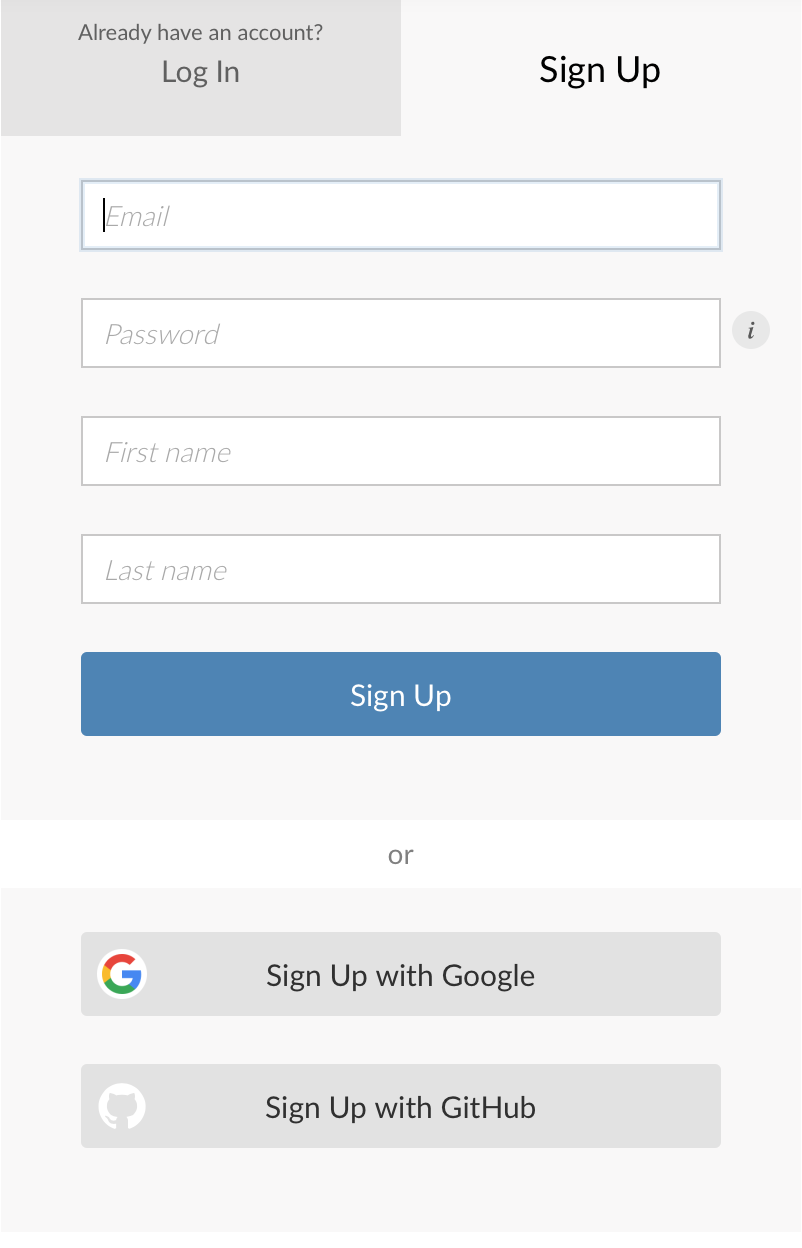
\includegraphics[width=1\linewidth]{_graphs/login.png}
  \caption{Création du compte}
  \label{login}
\end{subfigure}%
\begin{subfigure}{.5\textwidth}
  \centering
  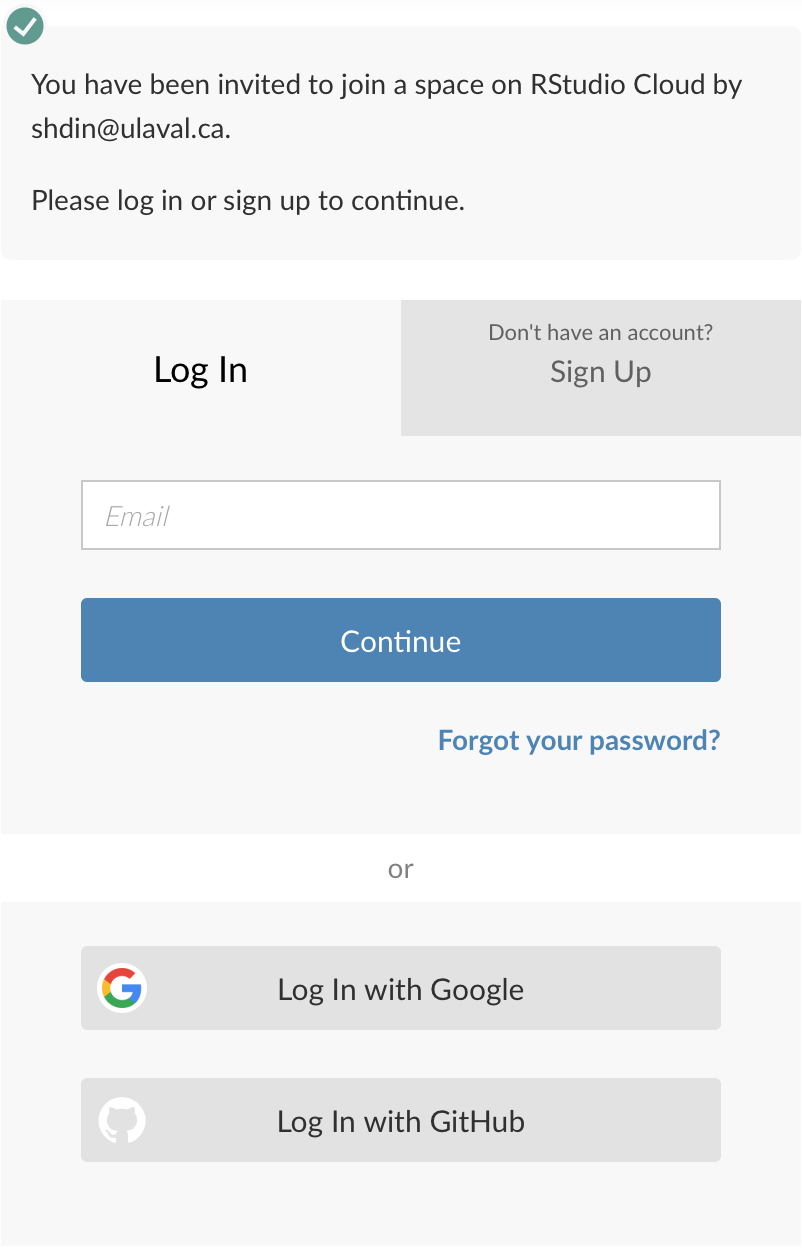
\includegraphics[width=1\linewidth]{_graphs/workspace.png}
  \caption{Inscription à l'environnement}
  \label{workspace}
\end{subfigure}
\caption{Connexion à \textbf{RStudio Cloud}}
\label{connexion}
\end{figure}
  
  \subsection{Interface}
  \textbf{RStudio Cloud} a deux interfaces, l'interface des espaces de travail et l'interface des projets. L'interface des espaces de travail est la première chose que vous rencontrez en vous connectant à \textbf{RStudio Cloud}. C'est ce qui vous permet de vous déplacer d'un projet à l'autre et d'un espace de travail à l'autre. La section \emph{menu} de cette interface offre aussi plusieurs liens à des ressources externes sur 1) l'utilisation de \textbf{RStudio Cloud}, 2) l'utilisation de \textbf{R} et 3) de ses \emph{packages} les plus populaires. Les figures \ref{home} et \ref{homeMenu} présentent un aperçu de l'interface des espaces de travail de \textbf{RStudio Cloud} et ses principaux points d'intérêt.
  
\begin{figure}[H]
  \centering
  \fbox{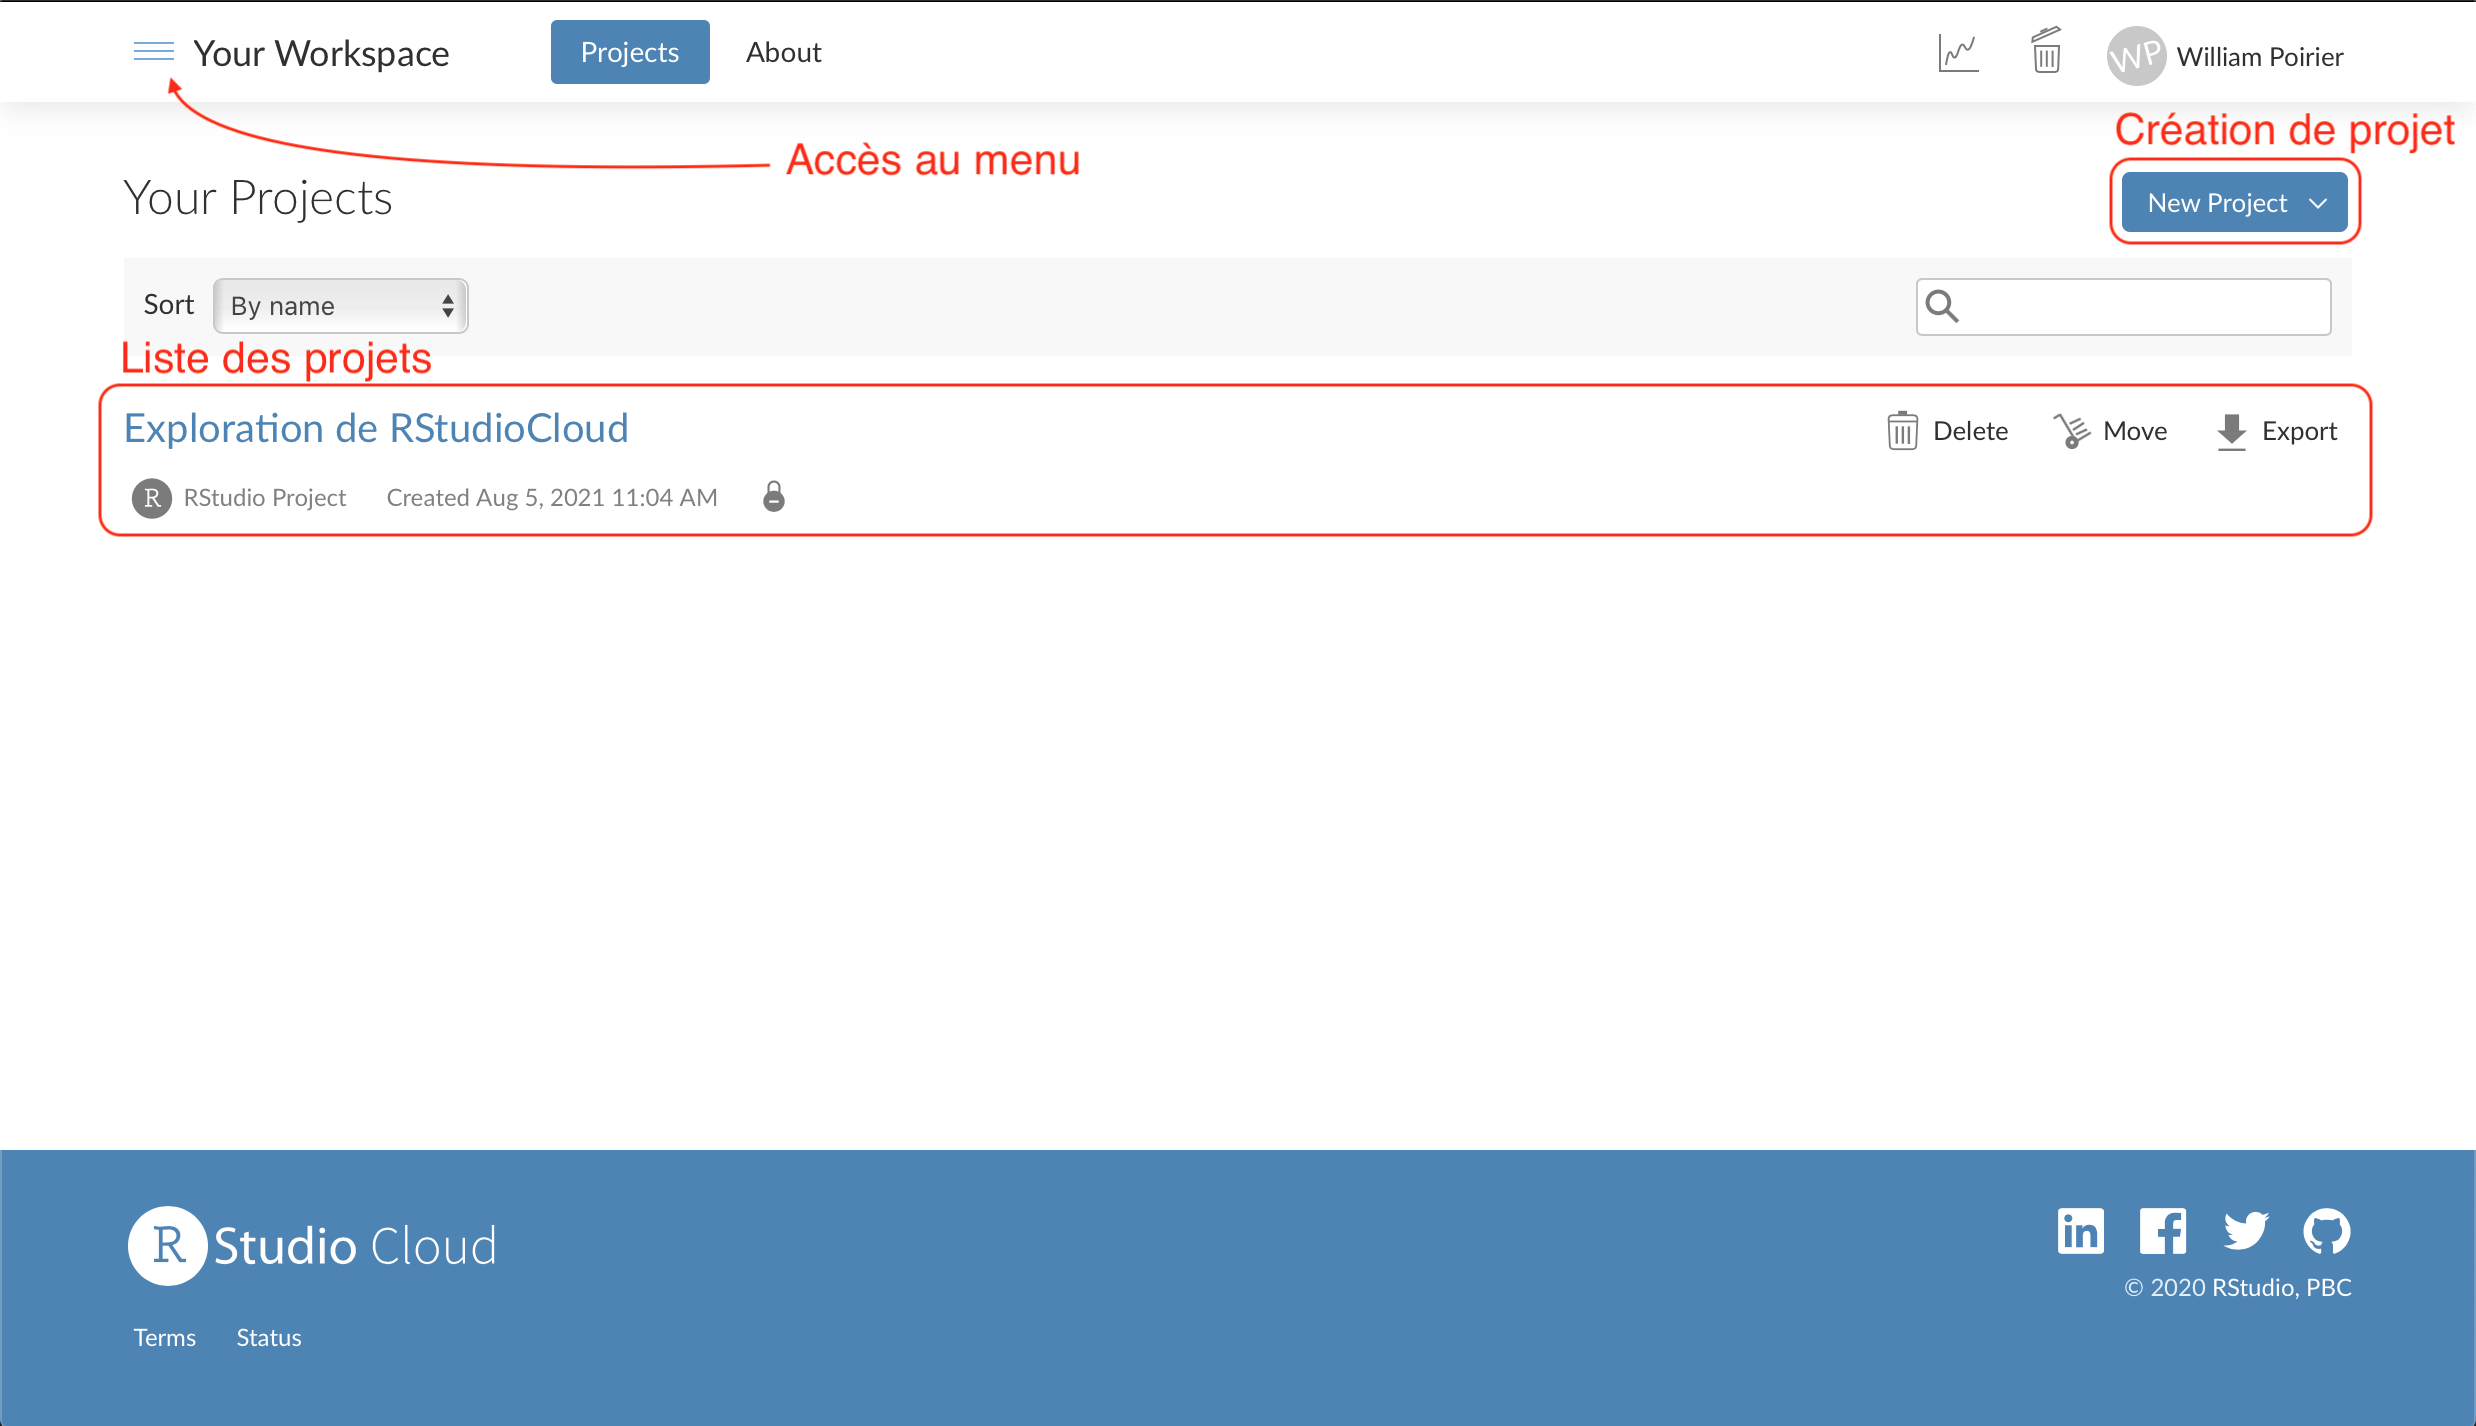
\includegraphics[width=1\linewidth]{_graphs/firstpage.png}}
  \caption{Page d'accueil}
  \label{home}
\end{figure}

\begin{figure}[H]
  \centering
  \fbox{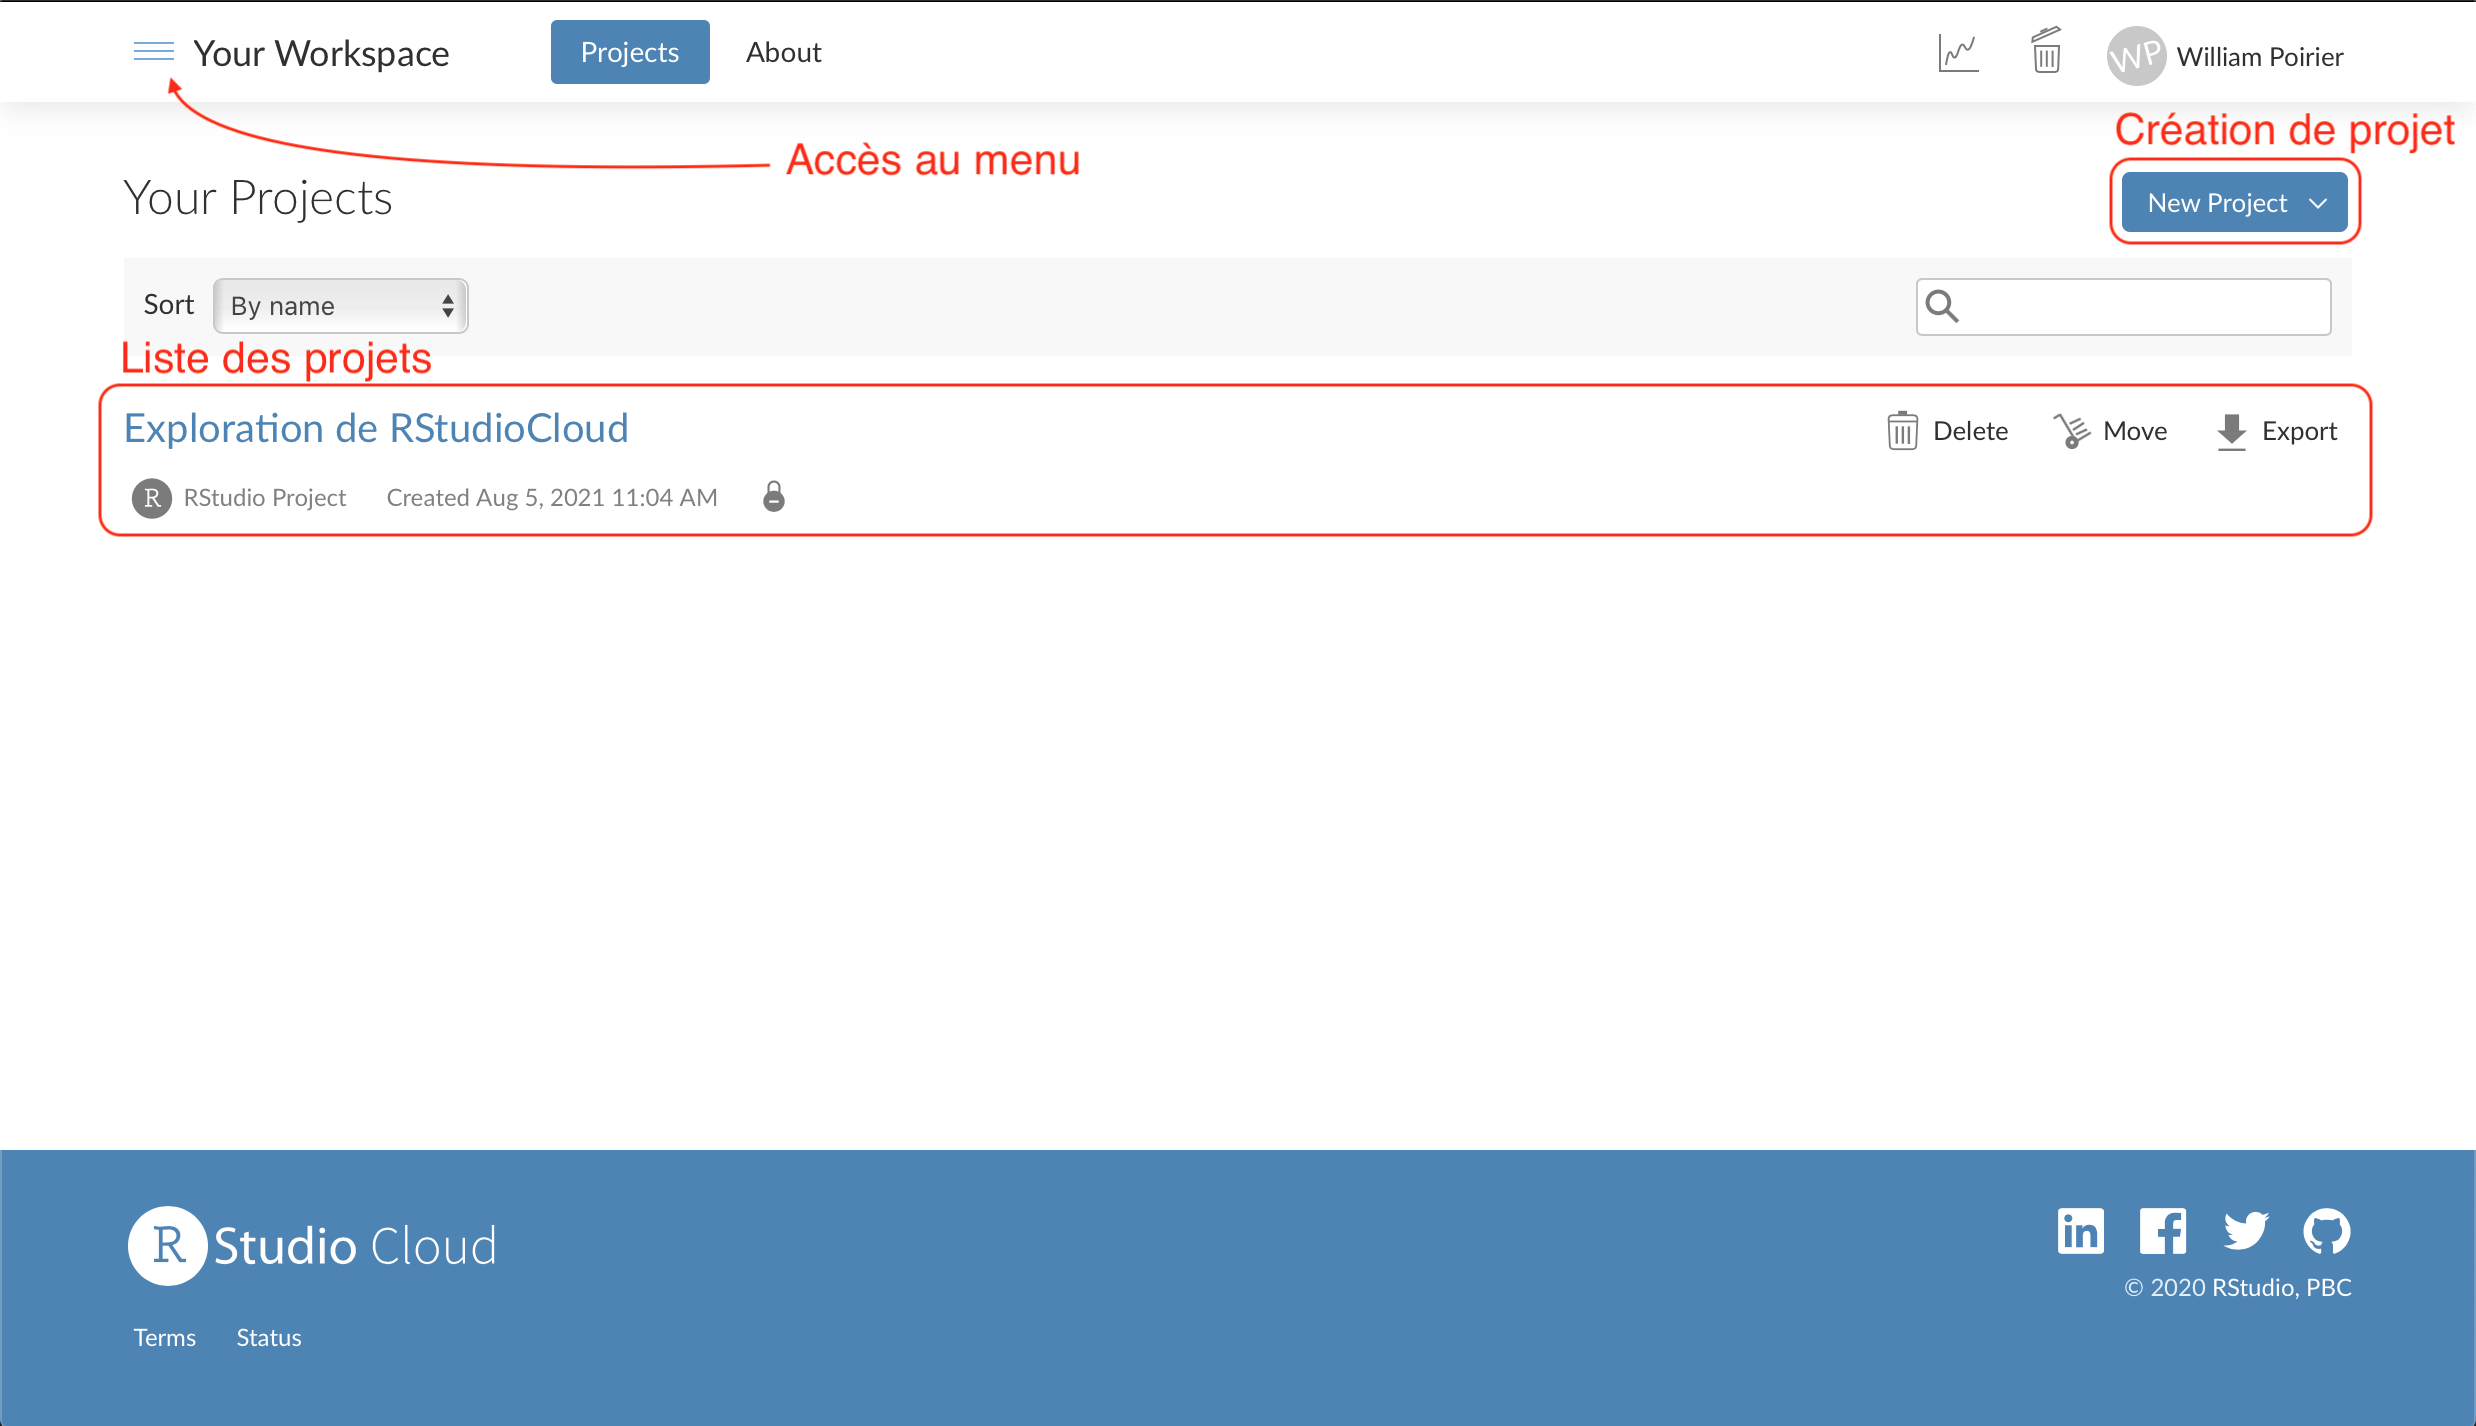
\includegraphics[width=1\linewidth]{_graphs/firstpage.png}}
  \caption{Menu d'accueil}
  \label{homeMenu}
\end{figure}

  La seconde interface est celle qui nous intéresse le plus, c'est où vous écrirez et exécuterez votre code. La figure \ref{rstudio1} présente les points d'intérêts les plus importants. L'\emph{environnement} contiendra les bases de données que vous importerez ainsi que tous les objets créés lors de la session\footnote{Ici, \emph{session} fait référence à la période de travail sur \textbf{RStudio Cloud}.}. Vous pouvez avoir accès à vos dossiers, les librairies utilisées, un aperçus des graphiques produits ainsi qu'à de l'aide dans la fenêtre en bas à droite. La plus grande fenêtre par défaut est celle contenant la console. La \textbf{console} est un environnement d'exécution directe. En d'autres mots, vous pouvez y écrire des commendes qui seront exécutées immédiatement. C'est utile pour faire des tests et exécuter de petite manipulation. Or, la \textbf{console} n'enregistre pas la suite de commende que vous lui demander de faire, ce n'est pas son rôle. Pour ce faire, il faut ouvrir l'\textbf{éditeur} tel que spécifié par la figure \ref{rstudio1}. L'\textbf{éditeur} c'est où l'on écrit un code (une suite de commandes permettant d'atteindre un but quelconque, comme la production d'un graphique) afin qu'il puisse être enregistré et réutilisé.  
  
\begin{figure}[H]
  \centering
  \fbox{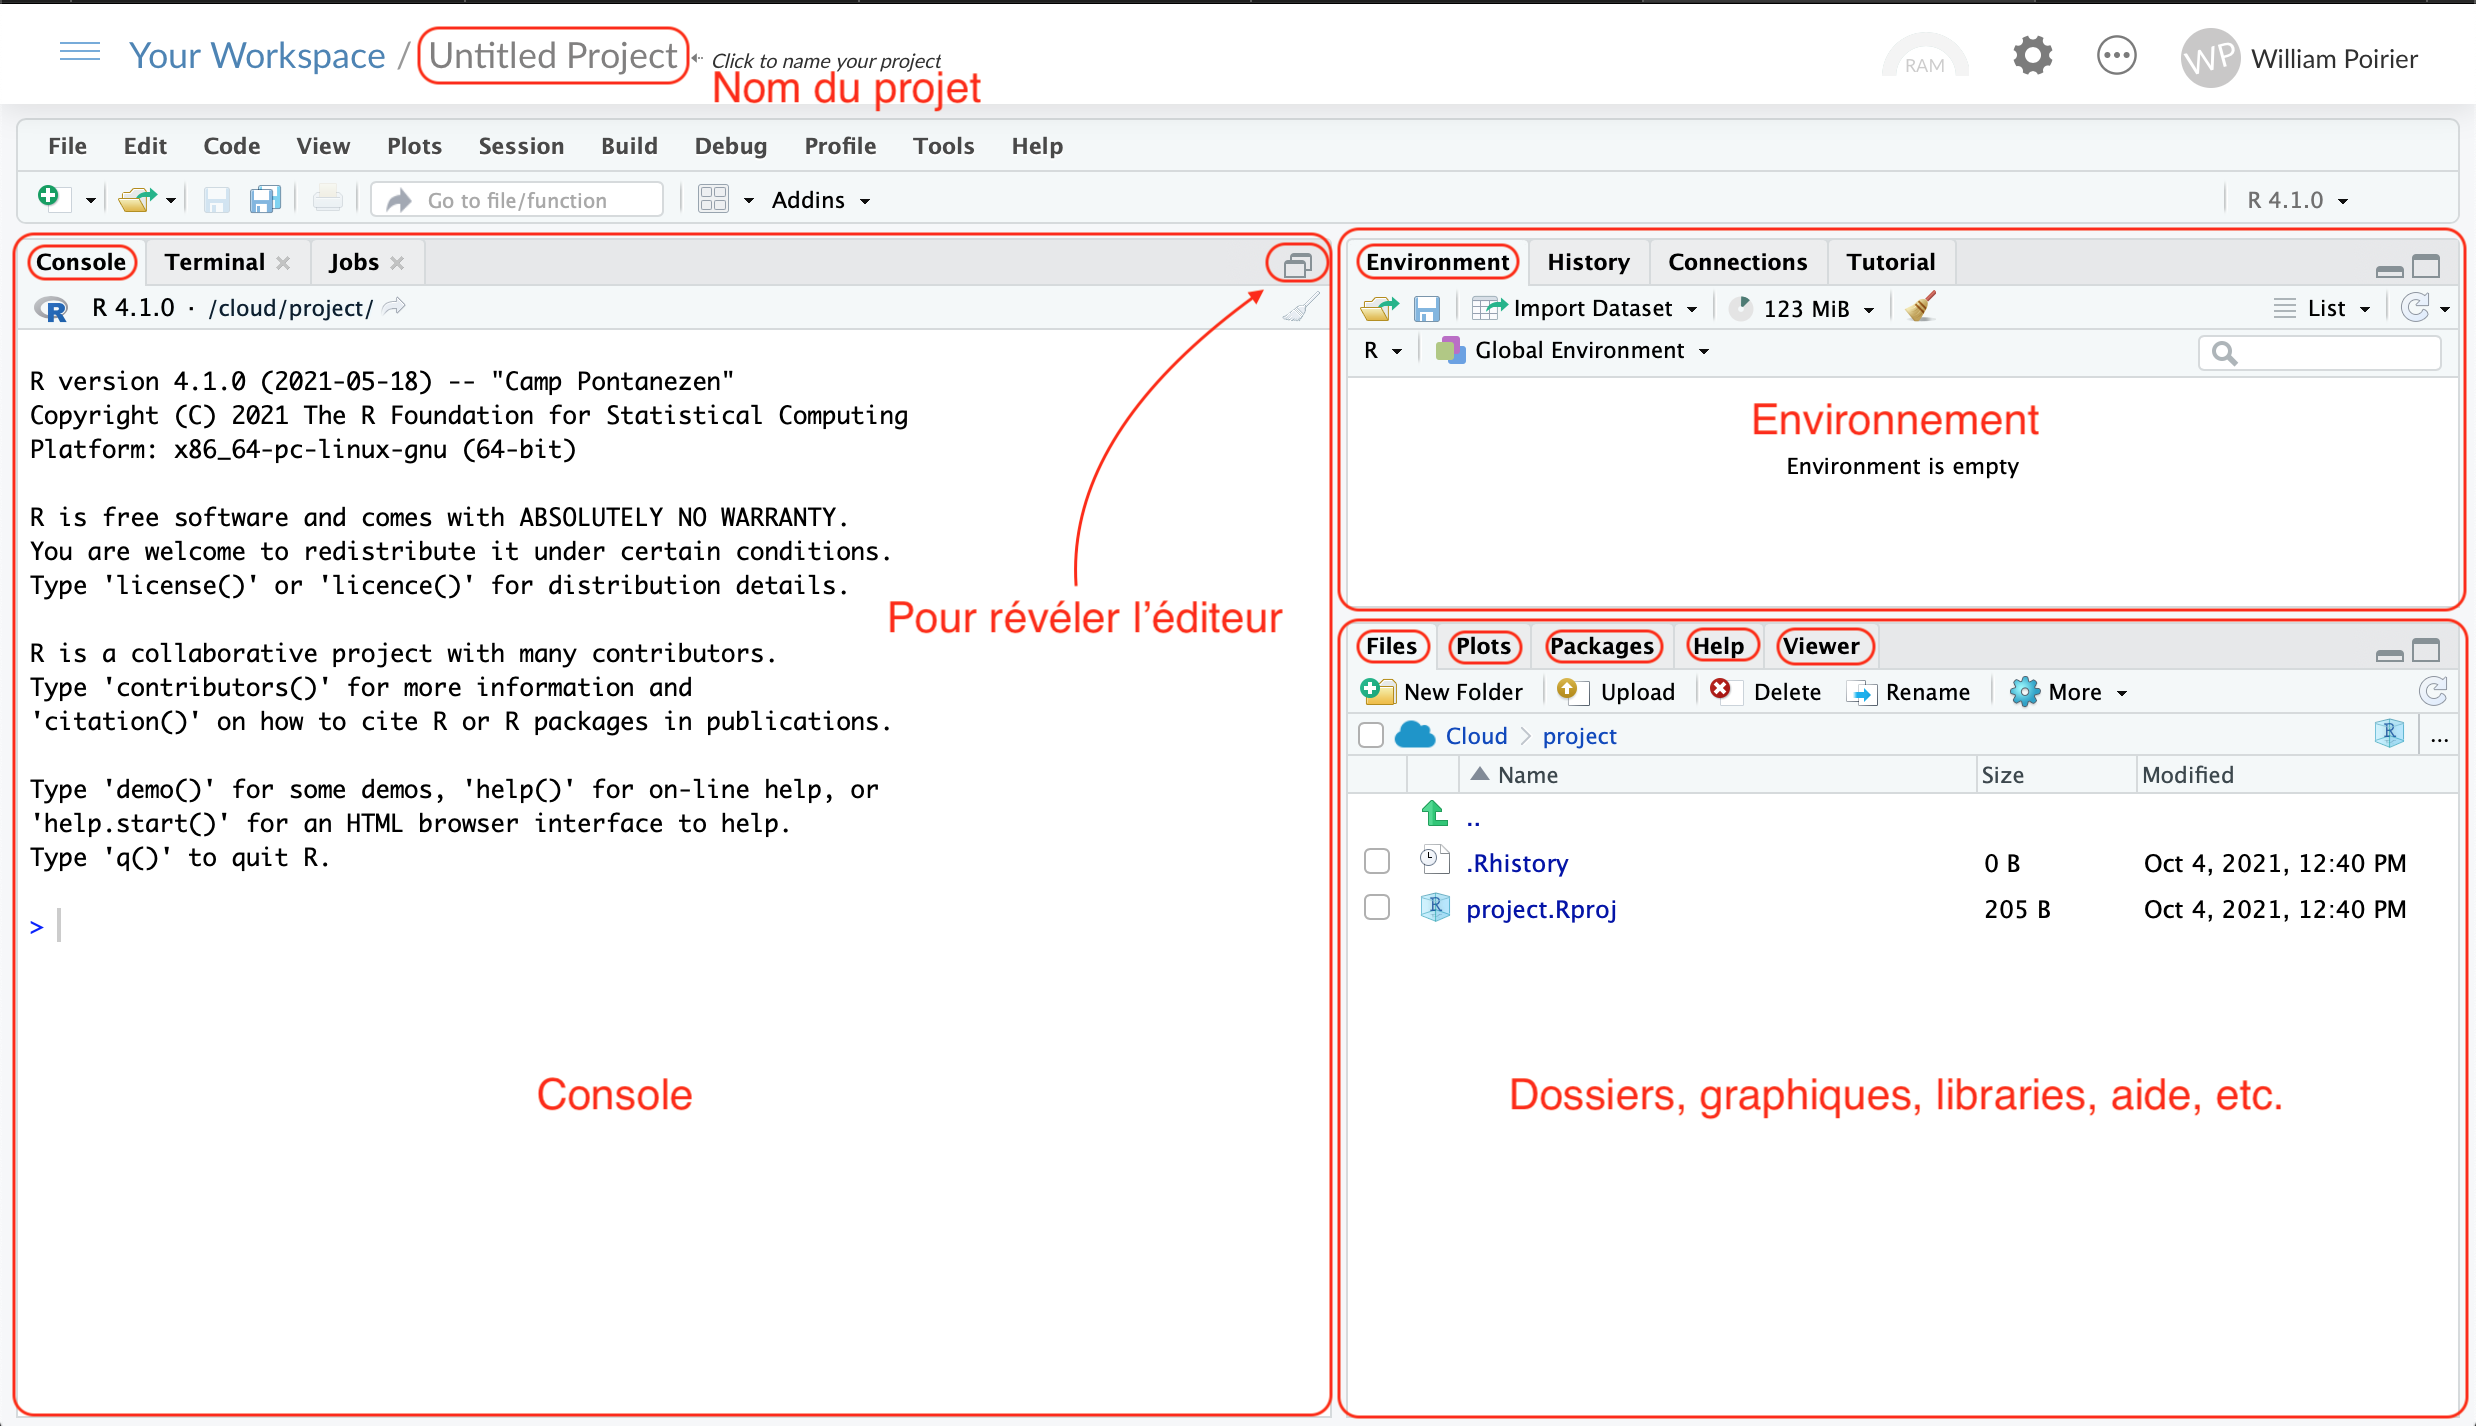
\includegraphics[width=0.98\linewidth]{_graphs/rstudio1.png}}
  \caption{État par défaut}
  \label{rstudio1}
\end{figure}

\begin{figure}[H]
  \centering
  \fbox{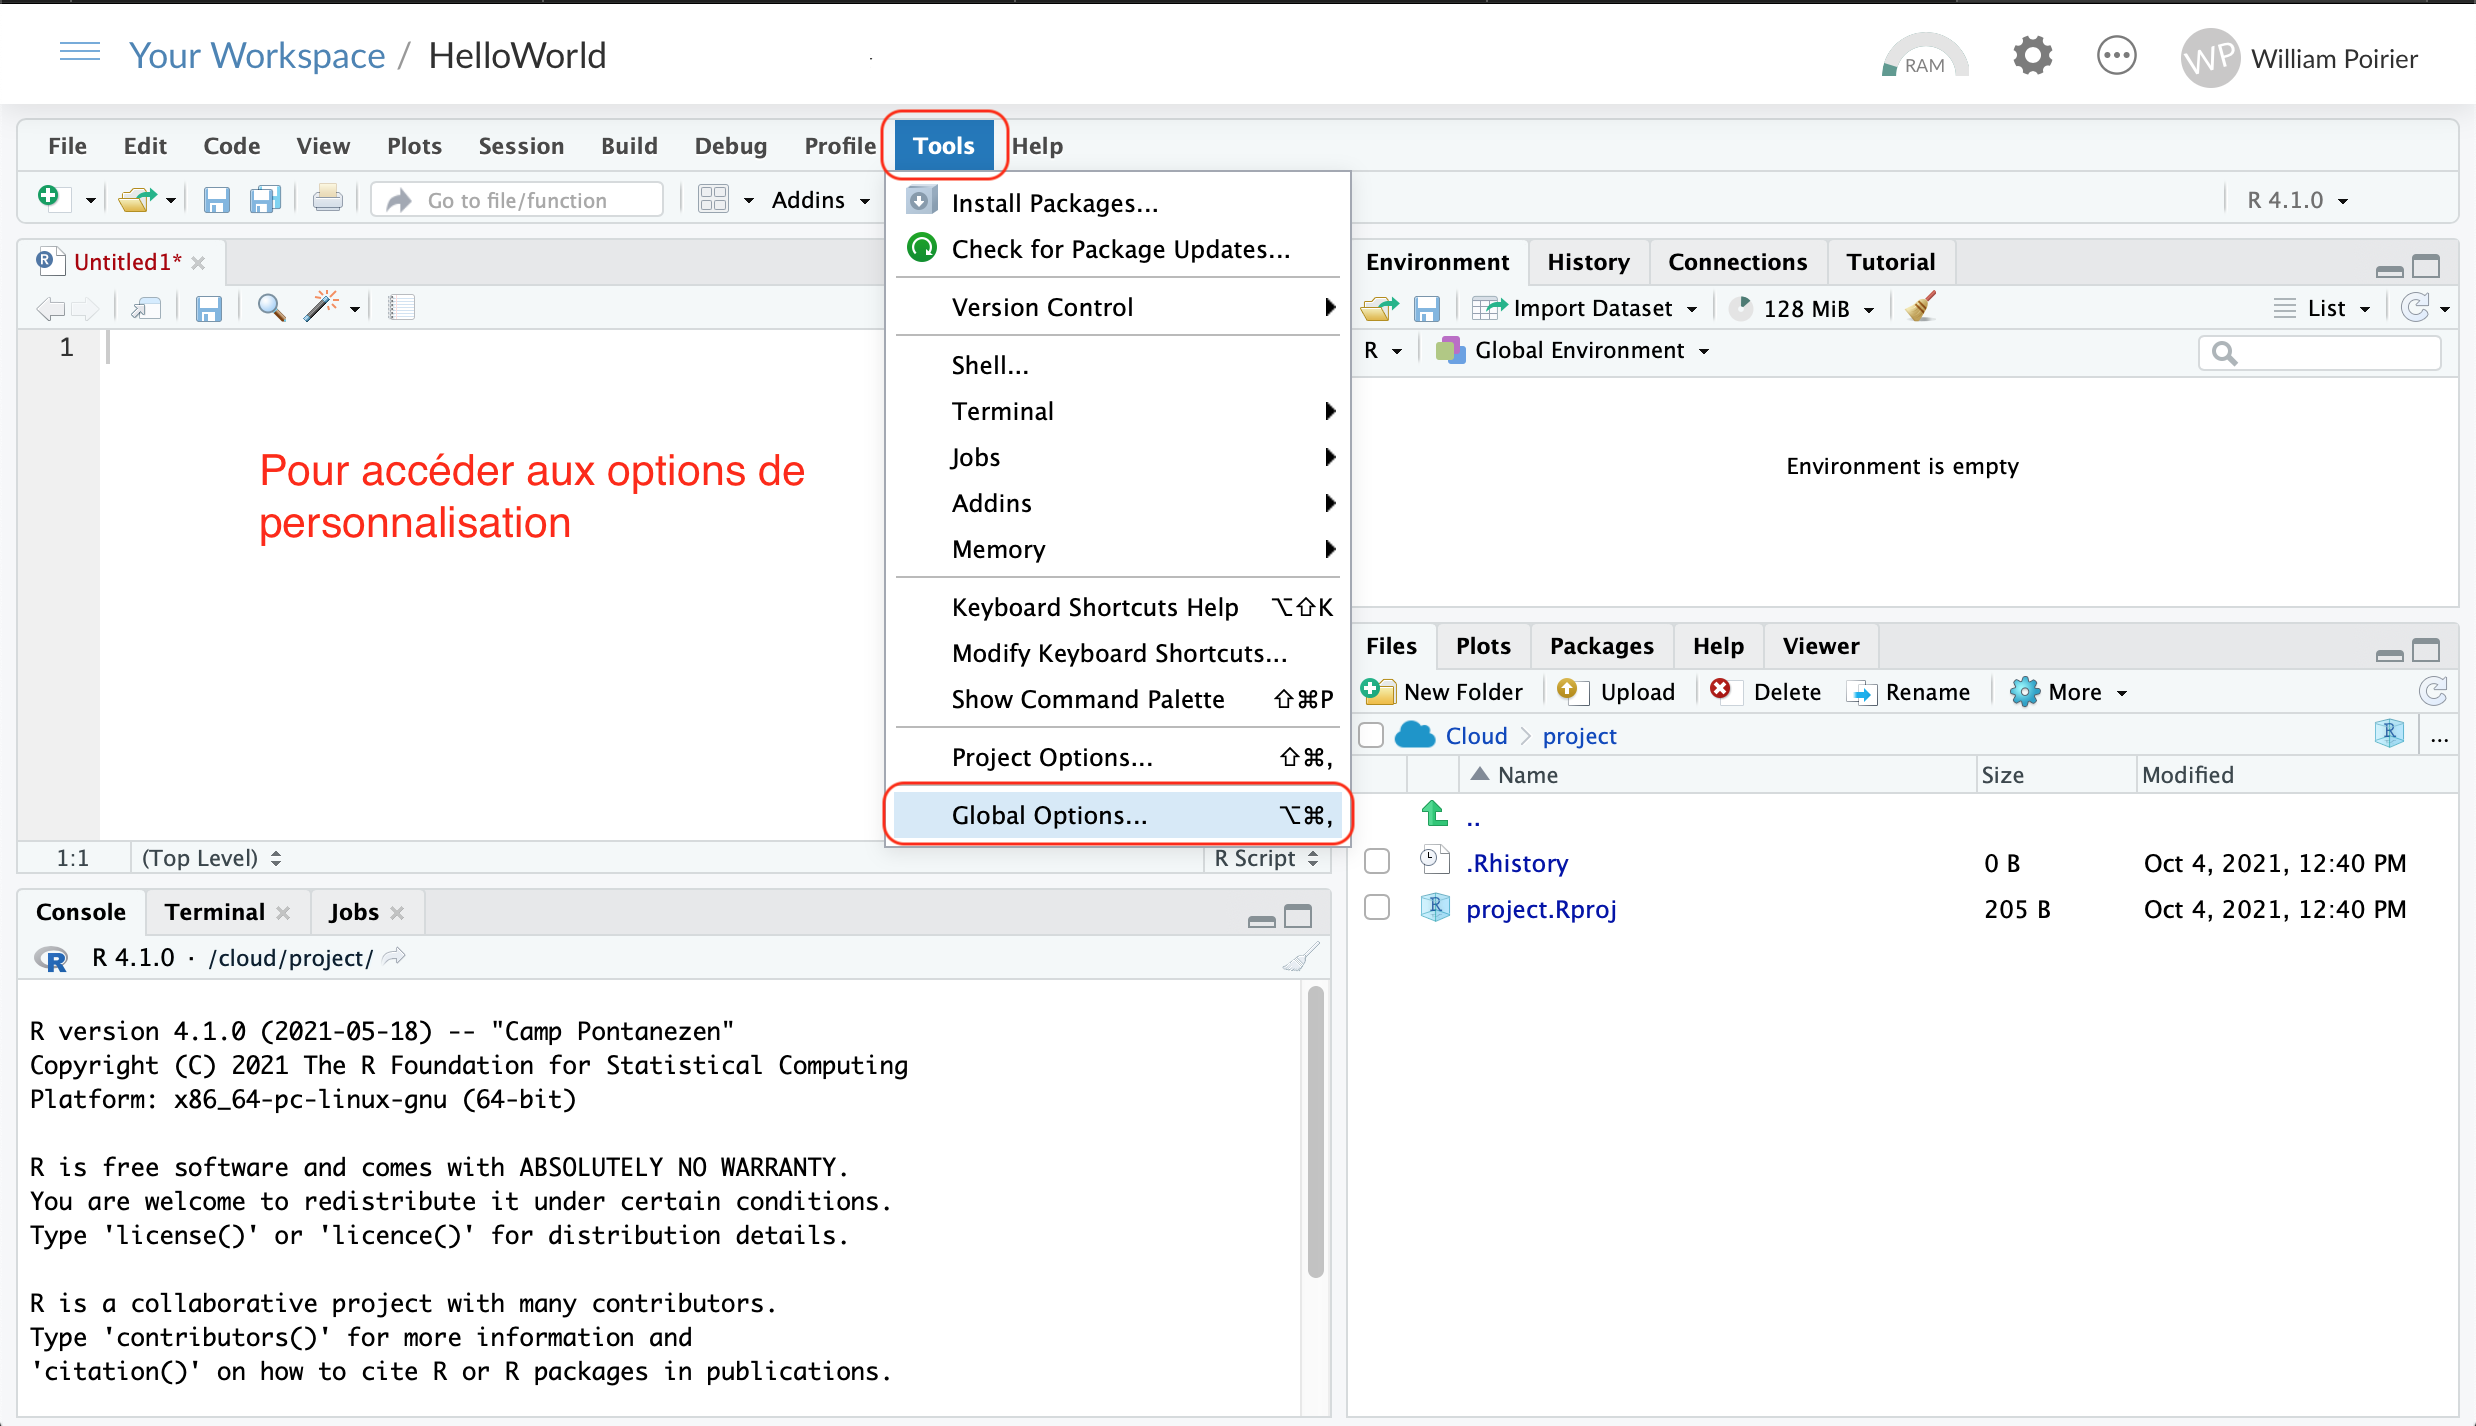
\includegraphics[width=0.98\linewidth]{_graphs/rstudio2.png}}
  \caption{Début de la personnalisation}
  \label{rstudio2}
\end{figure}

Avant d'entrer dans la syntaxe d'utilisation de \textbf{R}, je recommande fortement la personnalisation de votre environnement. Non seulement cela vous permettra d'avoir une expérience esthétique plus agréable, cela vous aidera à long terme à reconnaître les structures du langage. Les figures \ref{rstudio2} et \ref{rstudio3} montrent comment accéder aux options de l'environnement global. Vous y trouverez ma mise en place préférée. Je tends à préférer coder sur fond plus foncé, mais je vous encourage à explorer les options et à trouver ce qui vous correspond le mieux. C'est pour vos yeux, pas ceux de l'équipe d'enseignement. 

\begin{figure}[H]
  \centering
  \fbox{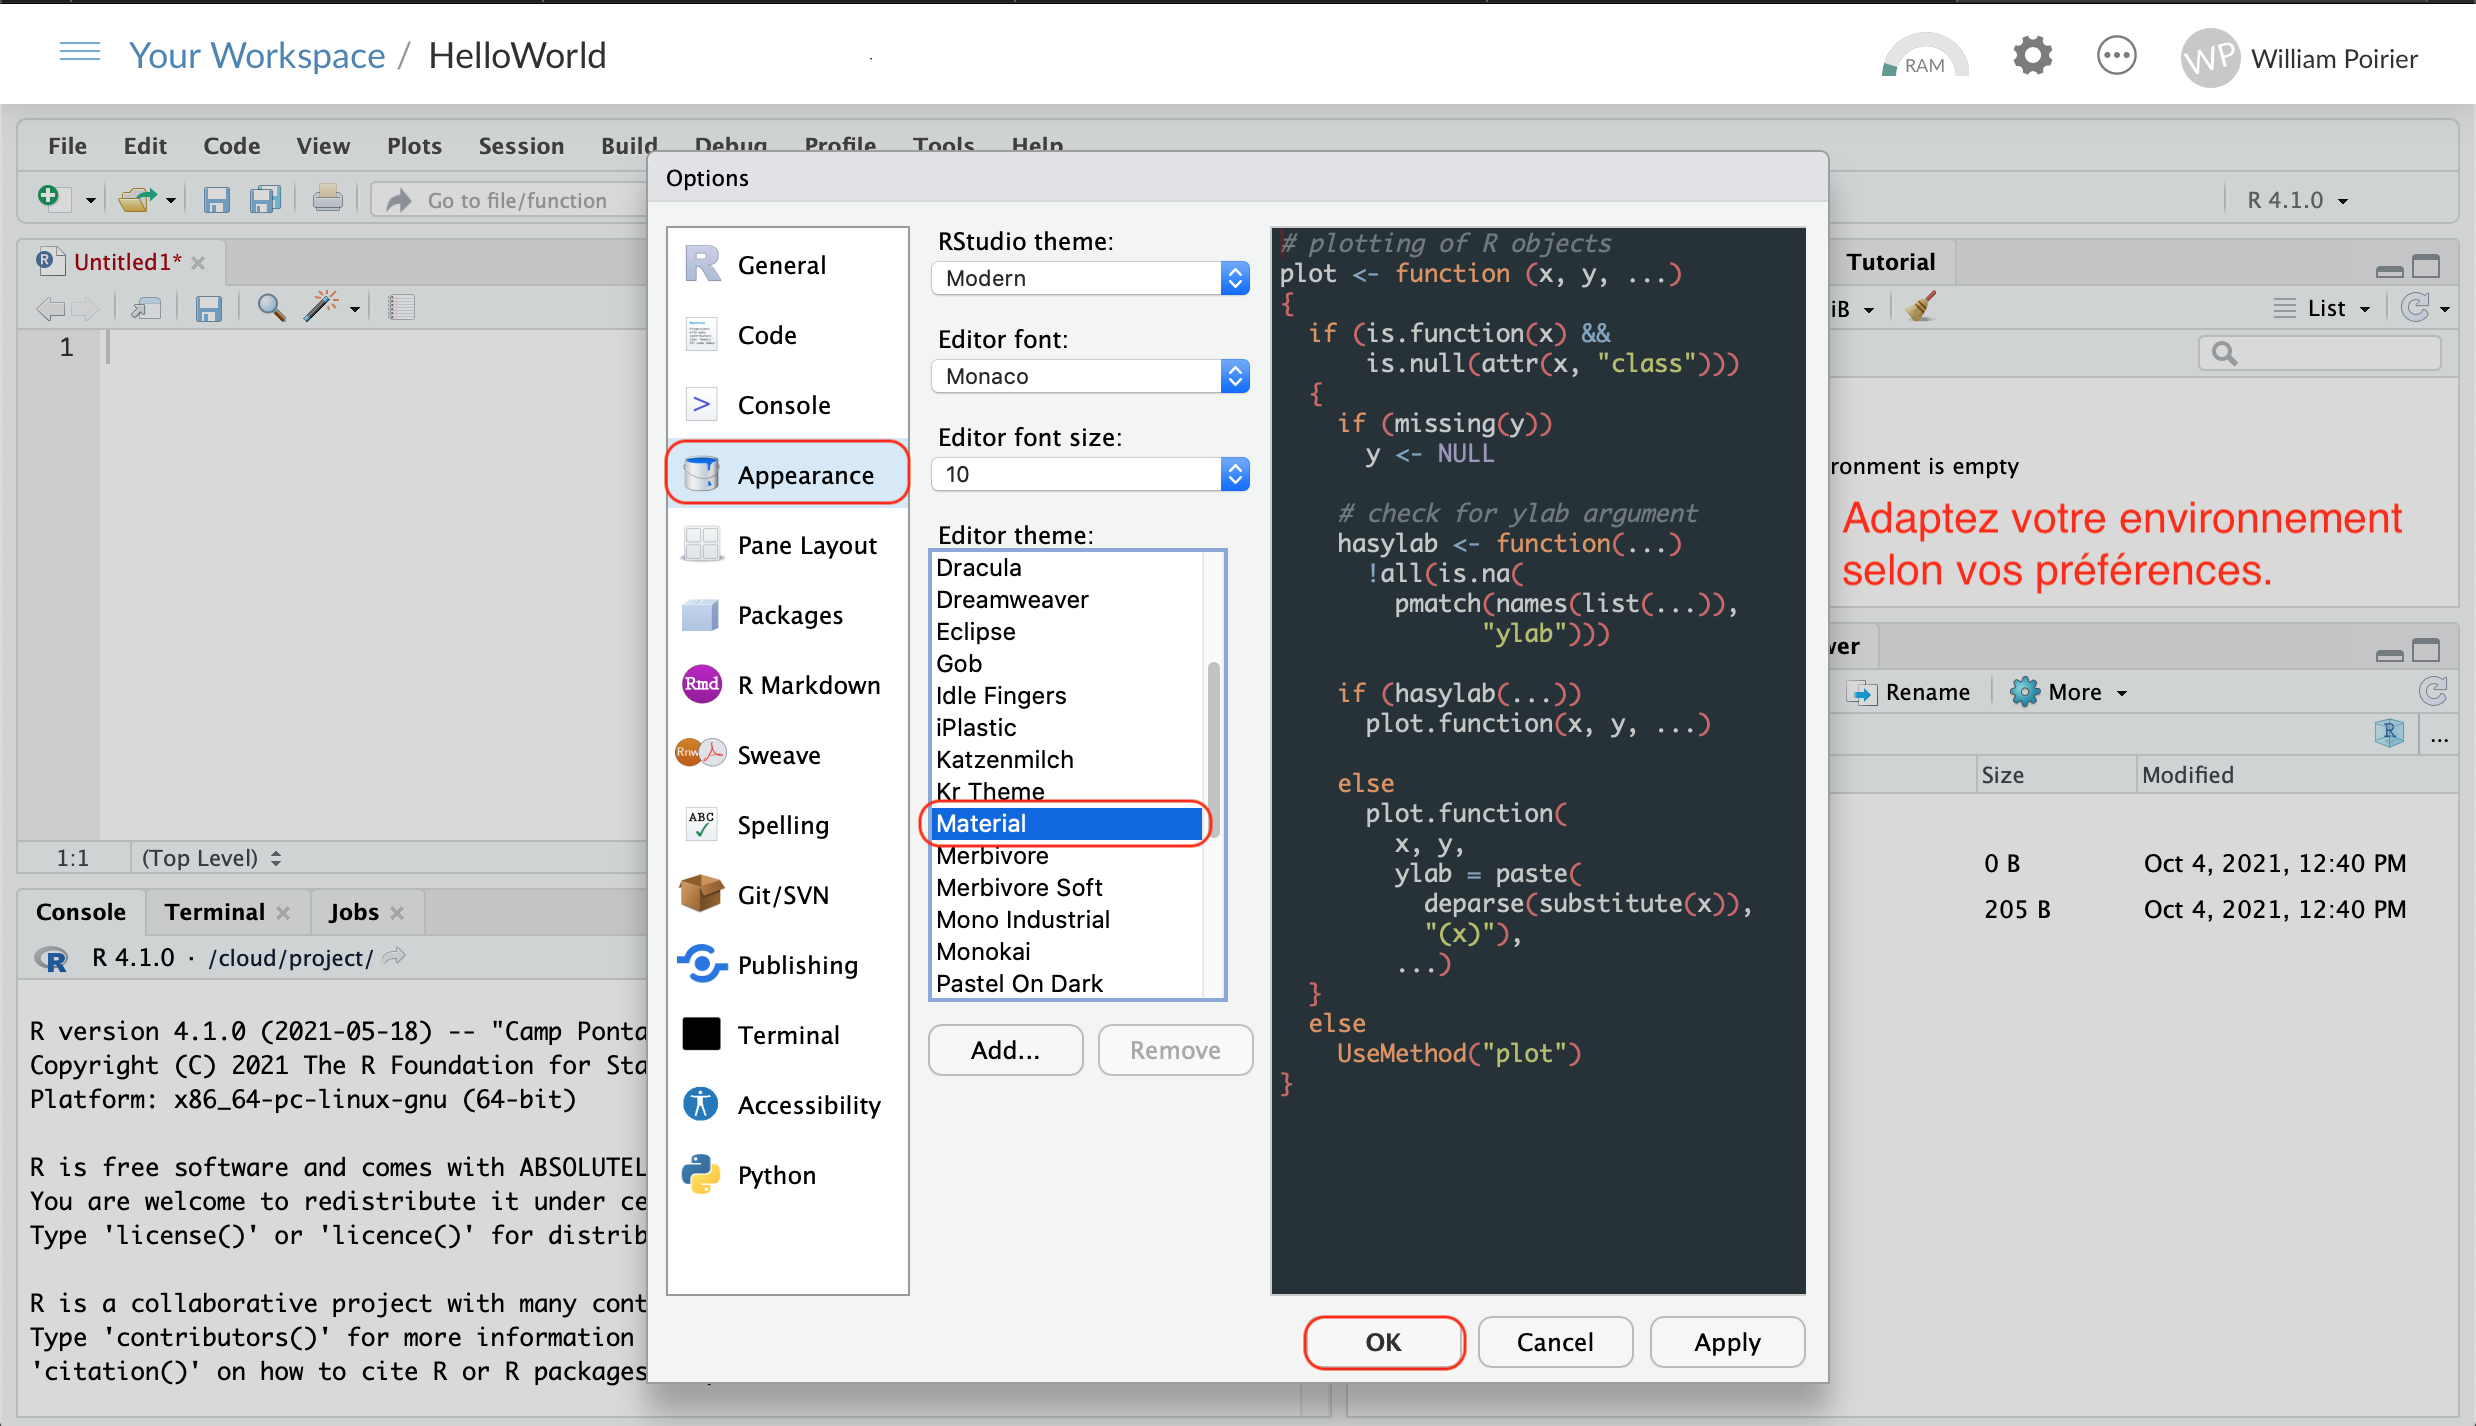
\includegraphics[width=0.98\linewidth]{_graphs/rstudio3.png}}
  \caption{Fin de la personnalisation}
  \label{rstudio3}
\end{figure}

\begin{figure}[H]
  \centering
  \fbox{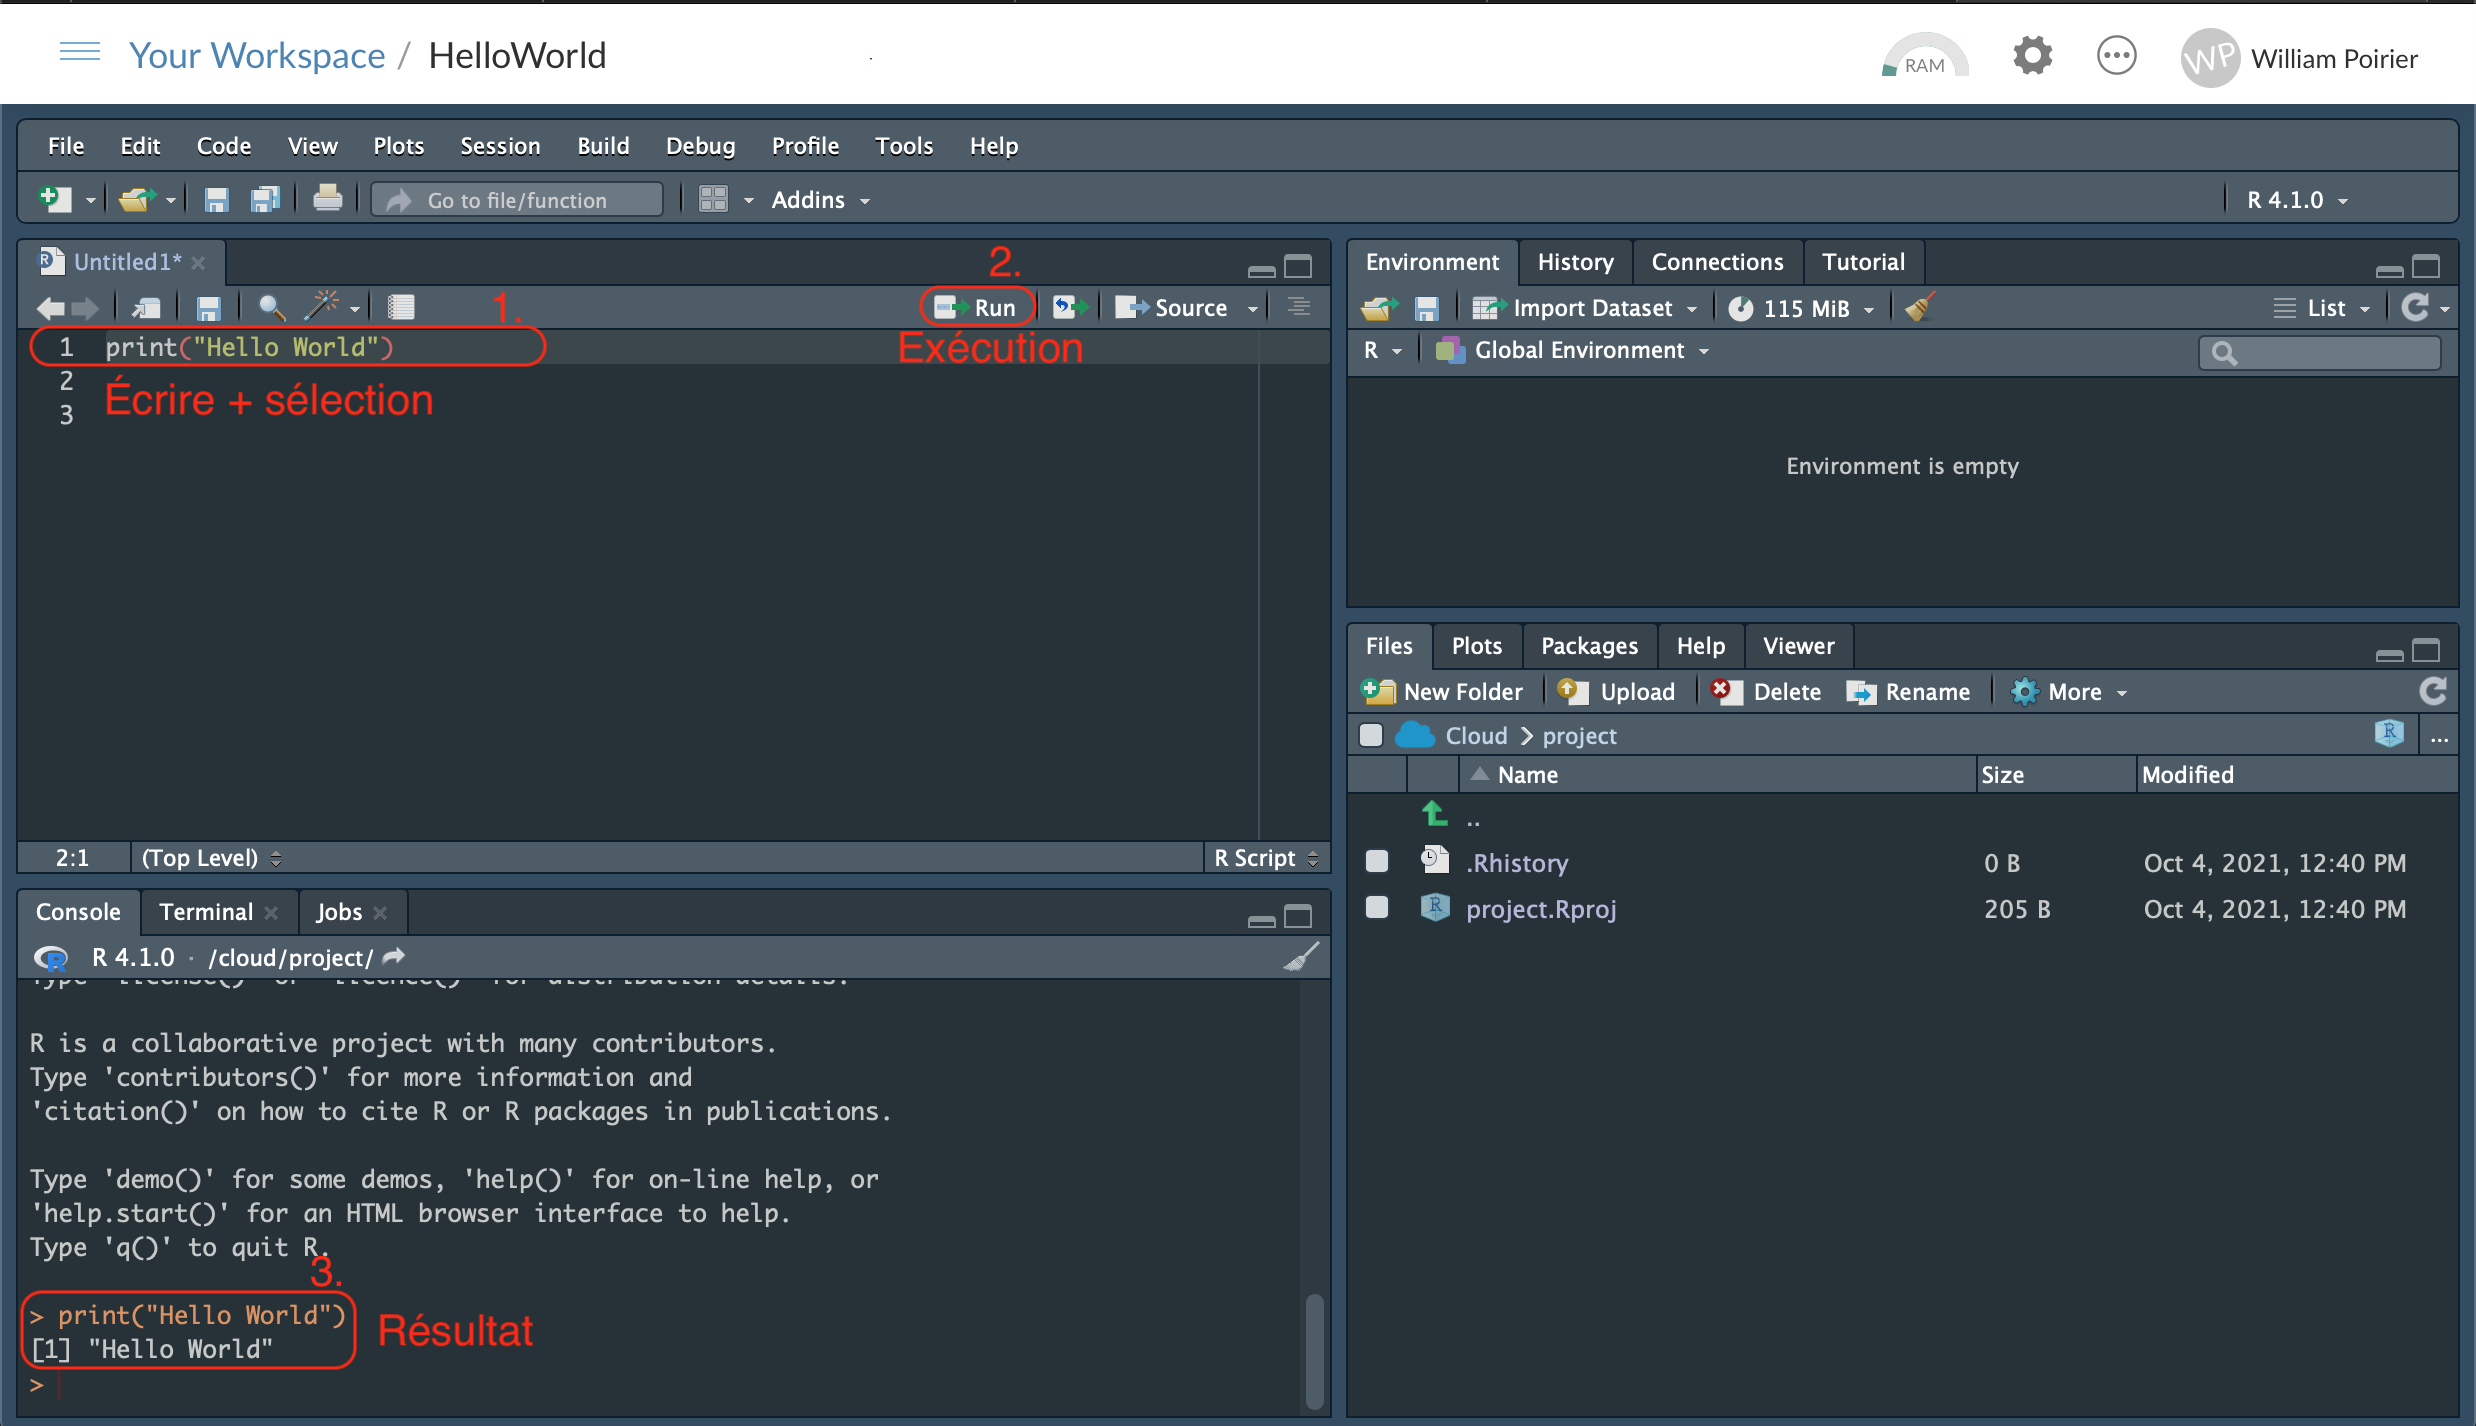
\includegraphics[width=0.98\linewidth]{_graphs/rstudio4.png}}
  \caption{Votre première ligne de code!}
  \label{rstudio4}
\end{figure}


\section{Hello World}

Vous vous apprêtez désormais à écrire votre première ligne de code. Allez dans l'éditeur, et tapez la commande suivante :
    \begin{lstlisting}
    > print("Hello World")
    \end{lstlisting}
À présent, il faut l'exécuter. Pour ce faire, sélectionnez la ligne, puis cliquez sur le bouton \textit{\textbf{RUN}} en haut à droite. La figure \ref{rstudio4} vous montre un exemple. Remarquez que le résultat s'affiche dans la console en bas. C'est sa deuxième utilité. La console vous indique les résultats des commandes que vous exécutez à partir de l'éditeur. Félicitation, vous êtes désormais des programmeurs, le fun peu commencer! 

  \subsection{Workflow}
  
  Un facteur important en prendre en considération lorsque l'on programme ou que l'on gère des bases de données, c'est l'organisation de notre «\emph{flux de travail}». Plusieurs facteurs sont à prendre en considération lorsque l'on veut optimiser son travail. Nous aborderons les principaux dans cette section.
  
    \subsubsection{Arborescence}
    Si vous avez lu le titre de la section et que vous ne savez pas ce à quoi nous faisons référence, ne vous inquiétiez pas, la plupart des gens utilisent l'arborescence de leur ordinateur sans s'en rendre compte. C'est tout simplement le chemin par lequel vous (ou votre ordinateur) doit passer pour accéder à un fichier. Comme quand vous voulez retrouver un vieux travail, votre ordinateur doit connaître où se trouvent les fichiers que vous mobilisez dans votre code. Pour se faire, il faut établir le «répertoire de travail» (\emph{working directory}) de la session \textbf{R}. On utilise alors la fonction \texttt{setwd()} et on y inscrit l'arborescence (le chemin) :
    
    \begin{lstlisting}
    # Pour les Mac
    > setwd("/Users/nomDelaSession/nomDuDossier/nomDuSousDossier")
    # Pour les PC
    > setwd("C:/Users/nomDelaSession/nomDuSousDossier")
    \end{lstlisting}
    
    Remarquez la façon dont l'arborescence est écrit. Chaque dossier est suivi d'une barre oblique (/) et d'un sous-dossier. C'est donc important de bien organiser les dossiers de sorte à éviter de devoir changer de répertoire de travail trop souvent. L'idéal c'est de référer à un dossier général contenant les dossiers spécifiques. Par exemple, vous pourriez avoir un dossier \texttt{ElectionFed21} qui contient un dossier \texttt{codeR}, un dossier \texttt{graphs} et un dossier \texttt{Data}. De cette façon, vous pouvez indiquer un répertoire de travail général au début de votre code pour ensuite utiliser des arborescence relative. Ne vous inquiétez pas, tout ceci s'éclairera durant la session.
    
    \subsubsection{Commentaires}
    
    Commenter un code c'est l'habitude la plus importante à prendre, surtout lorsqu'on est en apprentissage. Que voulons-nous dire par là? Imaginez que vous êtes en train d'explorer une forêt. Vous pourrez sans doute retrouver votre chemin de mémoire, mais l'idéal c'est de laisser des repères le long du chemin. Surtout si vous n'y retournez pas avant un moment. Coder c'est la même chose. Vous allez développer une suite d'instruction logique qui permettra de produire un résultat spécifique. Il faut donc vous assurer de pouvoir bien comprendre les différentes étapes de votre code, et ce, même après plusieurs mois ou années. La mémoire étant une faculté qui oublie, ce n'est peut-être pas l'outil le plus fiable pour cette tâche. Donc, pour commenter, il vous suffit de précéder ce que vous écrivez par un «$\#$» comme ceci :
    
    \begin{lstlisting}
    # Separation en trois niveaux de la variable ses_health
    > Data$ses_health[Data$ses_health==0.75 | Data$ses_health==1] <- 1 
    > Data$ses_health[Data$ses_health==0.5] <- 0.5
    > Data$ses_health[Data$ses_health==0.25 | Data$ses_health==0] <- 0
    \end{lstlisting}
    
    \subsubsection{Raccourcis clavier}
    
    Comme dans toute chose, avec de l'expérience, vous allez acquérir de la rapidité en codant. Or, certains raccourcis clavier de \textbf{RStudio} et \textbf{RStudio Cloud} pourrons vous éviter de perdre de précieuses secondes. Ceux-ci varient en fonction du système d'opération de votre ordinateur, les deux prochaines sections s'adressent donc aux utilisateurs Mac et PC respectivement. 
    
      \paragraph{Raccourcis clavier -- Utilisateurs Mac}
      \begin{enumerate}
        \item \texttt{cmd + enter}, permet de rouler la partie du code sélectionnée.
        \item \texttt{alt + sélection}, permet de sélectionner une portion de plusieurs lignes en même temps. Voir la figure \ref{altSelect}.
        \item \texttt{shift + flèches}, permet de sélectionner à l'aide des flèches (gauche, droite, bas, haut) du clavier.
        \item \texttt{cmd + flèches}, permet d'accéder au début (avec la flèche du haut) et à la fin (avec la flèche du bas) d'un document.
        \item \texttt{alt + flèche}, permet d'inverser une ligne avec celle du haut (avec la flèche du haut) ou avec celle du bas (avec la flèche du bas).
      \end{enumerate}
      
      \begin{figure}[H]
      \centering
      \fbox{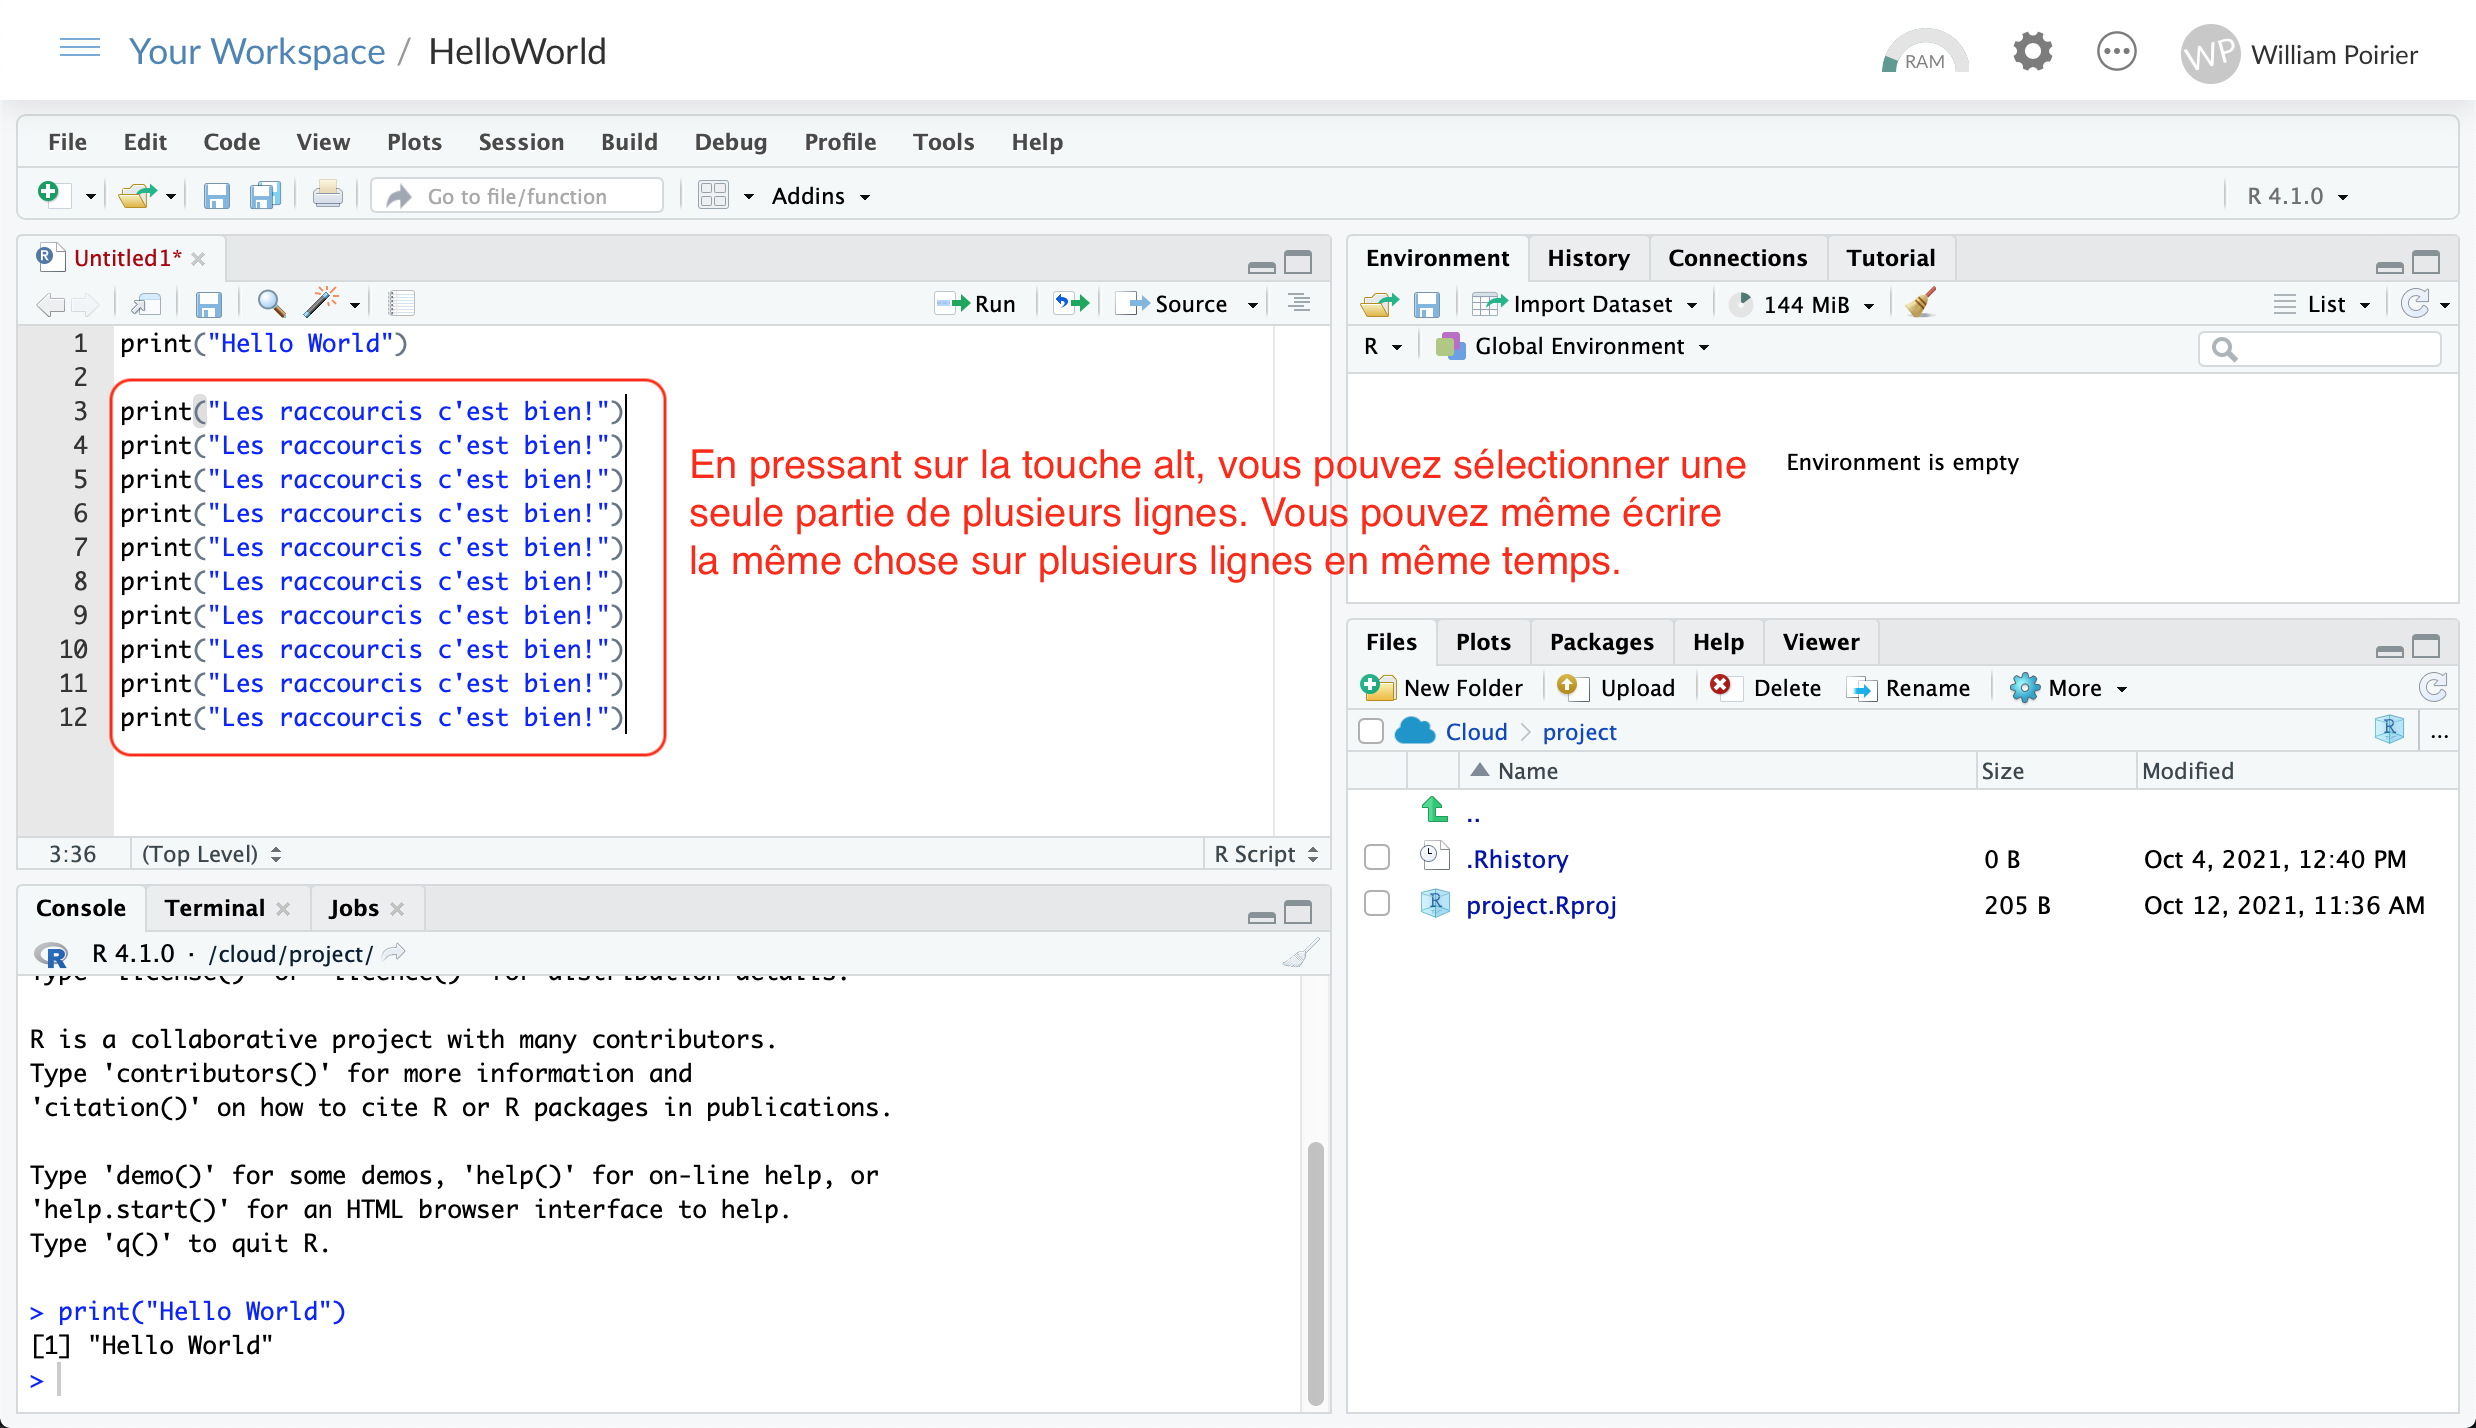
\includegraphics[width=0.98\linewidth]{_graphs/altSelect.png}}
      \caption{Sélection multiple de lignes}
      \label{altSelect}
      \end{figure}
      
      \paragraph{Raccourcis clavier -- Utilisateurs PC}
      \begin{enumerate}
        \item \texttt{ctrl + enter}, permet de rouler la partie du code sélectionnée.
        \item \texttt{alt + sélection}, permet de sélectionner une portion de plusieurs lignes en même temps. Voir la figure \ref{altSelect}.
        \item \texttt{shift + flèches}, permet de sélectionner à l'aide des flèches (gauche, droite, bas, haut) du clavier.
        \item \texttt{ctrl + flèches}, permet d'accéder au début (avec la flèche du haut) et à la fin (avec la flèche du bas) d'un document.
        \item \texttt{alt + flèche}, permet d'inverser une ligne avec celle du haut (avec la flèche du haut) ou avec celle du bas (avec la flèche du bas).
      \end{enumerate}

\section{Intro à la programmation en R}
Nous pouvons désormais entrer dans le vif du sujet, la programmation en \textbf{R}. Que vous utilisiez \textbf{RStudio}ou \textbf{RStudio Cloud}, les prochaines indications ne changent pas. 

  \subsection{Ça va bien aller}
  Plusieurs étudiants sont anxieux face à la tâche d'apprendre un langage de programmation. C'est tout à fait normal. La programmation vient avec une aura cryptique, un jargon et des programmeurs qui ne sont pas toujours à même d'expliquer ce qu'ils font. Or, pour ce cours, nous nous considérerons \textbf{R} comme une calculatrice +, c'est-à-dire d'un outil permettant d'effectuer des opérations mathématiques plus ou moins complexes. Vous ne deviendrez pas des développeurs à la fin de ce cours et ce n'est pas l'objectif. Le but est plutôt de vous former pour que vous soyez en mesure d'effectuer des analyses de bases, une compétence qui vous distinguera sur le marché du travail.

Ceci étant dit, vous allez avoir besoin d'aide à un moment c'est certains. L'équipe d'enseignement est bien entendue disponible pour répondre à vos questions. Cependant, nous préférons que vous développiez votre autonomie. Pour ce faire, nous vous encourageons à consulter les ressources en ligne mentionnée à la section \ref{R vs RStudio vs RStudio Cloud}. D'autres ressources sont également offertent par \textbf{R} lui-même. En précédent toute fonction d'un «?» dans la console\footnote{Lorsqu'une fonction n'est pas dans votre environnement de travail et que vous utilisé \texttt{?ggplot()}, \textbf{R} retournera une erreur du genre «\textcolor{BlueViolet}{\texttt{Error in .helpForCall(topicExpr, parent.frame()) : no methods for ‘ggplot’ and no documentation for it as a function}}». Lorsque c'est le cas, vous pouvez précéder la fonction d'un double «?». Ceci indiquera à \textbf{R} de chercher dans toute la documentation des serveurs de CRAN.}:

  \begin{lstlisting}
    # Dans la console, pour obtenir de l'aide pour la fonction sample()
    > ?sample()
  \end{lstlisting}
  
  \subsection{Opérateurs}
  Les différents types d'opérateurs sont la base de la programmation en \textbf{R}. C'est en manipulant ces opérateurs qu'il est possible de calculer une moyenne, de faire un graphique, ou de faire de l'apprentissage machine. Les prochaines sections vous présenteront aux opérateurs de bases auxquels vous allez avoir affaire dans le cadre du cours. 
  
    \subsubsection{Opérateurs de calcul}
    Les opérateurs de calcul sont les opérateurs mathématiques que vous connaissez (+,-,*,/). Il existe aussi l'opérateur modulo (\%\%) qui permet de calculer le reste d'une division euclidienne. C'est pratique pour identifier si un nombre est un diviseur d'un autre nombre.  

      
    \subsubsection{Opérateurs d'assignement}
    Les opérateurs d'assignement, comme leur nom l'indique, permettent d'assigner des valeurs à des objets. Deux options s'offrent à vous. Vous pouvez utiliser le signe d'égalité (=), mais il est fortement recommandé d'utiliser la flèche d'assignement (<-). Pourquoi? Il s'agit d'un standard de bonne pratique. Souvent en programmation, il y a plusieurs façons d'arriver au même résultat. Les standards de bonne pratique nous permettent d'identifier les pratiques optimales sans avoir à comprendre pourquoi une pratique est meilleure qu'une autre dans toutes ces nuances. Pour ce cours, utilisez la flèche d'assignement (<-). Voir la figure XXX pour un exemple.

    
    \subsubsection{Opérateurs logiques}
    Les opérateurs logiques retournent l'une de deux valeurs, vrais ou faux. Ils sont donc utilisé pour comparer deux objets. Voici les principaux : 
    \begin{itemize}
      \item A < B    : A est plus petit que B
      \item A > B    : A est plus grand que B
      \item A <= B   : A est plus petit ou égale à B
      \item A >= B   : A est plus grand ou égale à B
      \item A == B   : A est égale à B
      \item A != B   : A n'est pas égale à B
      \item \&       : Une condition \textbf{ET} une autre condition
      \item |        : Une condition \textbf{OU} une autre condition
      \item A\%in\%B : A est contenu dans B
    \end{itemize}
    
    Pour éclaircir un peu, je vous invite à faire ce petit test en tentant de répondre par vous même à la comparaison, puis en les testant dans la console.
    

    
    \subsubsection{Instructions de contrôle}
    Les instructions de contrôle sont ce qui rend R beaucoup plus puissant que votre calculatrice. En effet, elles permettent d'automatiser des procédures et des calculs. Trois instructions de contrôle principales sont à retenir :
    
    \begin{itemize}
      \item \textbf{if} (\emph{condition}) \{\emph{suite d'opération}\}
      \item \textbf{else} \{\emph{suite d'opération}\}
      \item \textbf{for} (\emph{facteur d'itération}) \{\emph{suite d'opération}\}
    \end{itemize}
    
    Les instructions de contrôle sont souvent ce qu'il y a de plus difficile à apprendre lorsqu'on commence à programmer. Leur maîtrise n'est donc pas essentielle pour la réussite de ce cours. Il est cependant important que vous ayez connaissance de leur existence. Je vous donne donc le défi de bien comprendre ce qui se passe dans le script de l'exemple à la figure XXX. Vous remarquerez que les commendes \emph{if} et \emph{else} peuvent être combiné en \emph{else if} et ainsi former une suite d'instructions. Avec le code de la «\emph{for loop}», vous devriez être en mesure d'écrire un code vous permettant d'imprimer (\emph{print()}) une étoile (*), puis deux, puis trois, jusqu'à $X$. C'est un exercice un peu futile, mais qui vous permettra de bien comprendre la logique des boucles en \textbf{R}. 
  
  \subsection{Structure de données}
  Vous savez désormais comment effectuer des opérations de bases sur des objets. Or, pour ce faire, il vous faut des objets à exploiter. Ces objets peuvent prendre plusieurs formes ayant chacune des caractéristiques et fonctionnalités différentes qui les rendent plus ou moins adaptées à différent type d'utilisation. Vous verrez ici les trois formats principaux qui seront utilisés dans le cours. 
  
    \subsubsection{Types de données et constantes}
    Quatre types de données principales sont à maîtriser. Les données de classe \emph{caractère} (ou «\emph{character}») sont considérées comme du texte par \textbf{R}. Ils ne peuvent donc pas être sujets aux opérations mathématiques standard. Par exemple, la figure XXX présente l'objet \texttt{veggiesName} qui contient la valeur textuelle \emph{carotte}. Pour assigner une donnée textuelle, il faut l'encadrer de guillemets « "" ». Si vous exécutez la ligne 56 vous obtiendrez une erreur puisque l'opération demandée ne peut pas s'appliquer à la classe de l'objet. Chose importante, même s'il s'agit d'un chiffre, si vous l'encadrer de guillemets comme à la ligne 58, \textbf{R} considérera l'objet comme du texte et la même erreur se produira. 
    
    Pour faire des opérations mathématiques, il faut utiliser des valeurs numériques ou booléennes. Les valeurs numériques sont des chiffres. Ceci inclut les nombres entiers, rationnels ($\pi$ ou $e$), et décimaux. Les valeurs booléennes ont deux valeurs possibles et correspondent aux réponses possibles des opérateurs logiques, soit \texttt{FALSE} ou \texttt{TRUE}. Bien qu'à première vu les valeurs booléennes ressemblent à des données textuelles, \textbf{R} les comprends comme 0 et 1 respectivement. C'est pourquoi si j'additionne \texttt{tomatoFruit} et \texttt{potatoFruit} j'obtiens 1.
    
    Un format alternatif et particulier des données textuelles et numériques sont les \emph{facteurs}. Conceptuellement, un facteur en \textbf{R} est un objet pouvant prendre un nombre limité de valeurs. En d'autres mots, il s'agit d'une variable catégorielle. À ces valeurs il est possible d'imposer un ordre. Par défaut, \textbf{R} ordonnera les valeurs numériques en ordre croissant et les valeurs textuelles en ordre alphabétique. En utilisant la fonction \texttt{factor()}, il est possible de créer un objet de classe facteur et de lui imposer un ordre avec l'argument \emph{levels}. Si les facteurs vous semblent compliqués pour rien, ils vous seront très utiles lorsque vous voudrez faire de la visualisation de données plus avancée. Il s'agit également d'une source d'erreur importante. Assurez-vous donc de bien connaître la classe des objets avec laquelle vous travaillez.
    
    Il est possible de connaître la classe d'un objet en regardant ce qui se trouve à l'intérieur. Or, ce n'est pas toujours possible ou évident, soit à cause de la taille de l'objet (la quantité de choses qui s'y trouve), soit parce qu'on peut confondre un 1 caractère et un 1 numérique ou une "pomme" caractère ou une "pomme" facteur. Pour être absolument certain, il est toujours préférable de demander à \textbf{R} lui-même en utilisant la fonction \texttt{class()}.
    
    Les constantes sont des objets avec une seule donnée d'associée. À la figure XXX, \texttt{veggiesName}, \texttt{nbVeggies}, et \texttt{tomatoFruit} sont des constantes, un objet avec un seul élément. Ces constantes n'ont cependant pas la même classe -- soit, respectivement, caractère, numérique et booléen. Les constantes forment l'unité de base des structures de données possibles en \textbf{R}. 
    
    \subsubsection{Vecteurs}
    Vous avez sans doute déjà entendu parler de vecteurs dans vos cours de mathématiques au secondaire. N'ayez crainte, il n'est pas question de la même chose ici. Un vecteur pour \textbf{R} c'est une série de données du même type. En d'autres mots, c'est une suite de constantes de la même classe mises bout à bout. Vous en avez déjà rencontré sans l'avoir remarqué. À la figure XXX, \texttt{myFruitsNames} est un vecteur de classe caractère et de longueur 4. Pour déterminer combien d'éléments contient un vecteur (ou quelle est sa longueur, vous pouvez les compter vous-même ou demander à \textbf{R} de le faire pour vous avec la fonction \texttt{length()} comme c'est fait à la ligne XX de la figure XXX. 
    
    Pour créer un vecteur, il faut utiliser la fonction \texttt{c()} et l'assigner à un objet, comme à la ligne XX de la figure XXX. Le c de la fonction représente le verbe anglais «concatenate» qui signifie relier (beaucoup de choses) ensemble dans une chaîne ou une série. Vous pouvez également ajouter des noms aux éléments de votre vecteur. Ces noms n'auront aucune influence sur le traitement des valeurs associées. Par exemple, à la figure XXX, j'ai un vecteur avec le nombre de chaque type de fruits dans le bon ordre (\texttt{nbFruits}). Si je désire leur associer un nom pour ne pas oublier ce que chaque chiffre représente, je peux utiliser la fonction \texttt{names()} comme à la ligne XX de la figure XXX. Cette ligne ce lit comme suit : aux noms des éléments de \texttt{nbFruits}, assignes les valeurs qui se trouvent dans \texttt{myFruitsNames}. Vous pouvez également associer directement les noms de chaque élément à la création du vecteur comme à la ligne XX de la figure XXX. 
    
    À la ligne XX de la figure XXX, j'amande le vecteur \texttt{nbFruits} en y ajoutant un élément. Remarquez comment je réutilise l'objet \texttt{nbFruits} dans l'opération. La ligne XX se lit : associes à l'objet \texttt{nbFruits} un vecteur des valeurs déjà contenues dans \texttt{nbFruits} et la valeur "trois" au nom "concombre". Or, n'ai-je pas dit plus haut qu'un vecteur se devait d'avoir le même type de valeurs? \textbf{R} est gentil, il vous laisse le faire sans retourner d'erreur. À la place, il prend une décision pour vous en assignant la classe caractère à \textbf{TOUS} les éléments du nouveau vecteur. C'est donc important d'être attentif à ce que \textbf{R} fait, il prend parfois de mauvaises décisions pour vous. 
    
    \subsubsection{Data frames}
  
\section{Importation de données}
  \subsection{Logique de projet RStudio Cloud}
  \subsection{Type de fichier}
  \subsection{Domestication}

  
\section{Analyse - Description}
  \subsection{Univariée}
  \subsection{Bivariée}
  \subsection{Visualisation}


\section{Analyse - Régression}
  \subsection{Linéaire}
  \subsection{Linéaire multiple}

  
\section{Pour aller plus loins}
 
%\section{Bibliographie}
%\begingroup
%\renewcommand{\section}[2]{}
%\bibliographystyle{apacite}
%\bibliography{mybibfile.bib}
%\vspace{10cm}
%\endgroup

\end{document}